% =============================================================
% Lectures 10 + 11 combined: Classical Tests, ANOVA & A/B Testing
%
% Pedagogical structure (Option B — instance first, theory at end):
%   Parts I-IV: named tests as recipes (t-tests, proportions, chi-squared,
%               nonparametric), then the decision flowchart + Python.
%   Part  V:    LRT framework REVEALED at the end — students have seen
%               the patterns, so restricted/full and Wilks make sense.
%   Parts VI-IX: ANOVA, A/B testing, pitfalls, big picture (formerly L11).
%
% Other improvements over the previous version:
%   - one-sample t-test now reports a p-value, not just critical value
%   - two-sample t-test gets a tight worked example (Teaching Methods)
%   - chi-squared distribution introduced as "sum of squared standardised
%     errors" — connects to MSE/RSS instead of arriving as the limit of
%     -2 log Lambda
%   - Wilcoxon example uses mixed-sign differences (not all positive)
%   - Mann-Whitney rank visualization simplified to a clean table
%   - SS decomposition paired with concrete numbers
%   - flowchart "ANOVA (Part VI)" forward-ref updated to "ANOVA (later)"
% =============================================================

\documentclass[aspectratio=169]{beamer}

\usetheme{default}
\usecolortheme{dove}

\setbeamertemplate{navigation symbols}{}
\setbeamertemplate{footline}{%
  \hfill{\large\insertframenumber\,/\,\inserttotalframenumber}\hspace{0.8em}\vspace{0.5em}%
}

\definecolor{popblue}{RGB}{52, 101, 164}
\definecolor{sampred}{RGB}{204, 0, 0}
\definecolor{paramgreen}{RGB}{0, 140, 70}
\definecolor{warnred}{RGB}{180, 40, 40}
\definecolor{orange1}{RGB}{220, 120, 0}
\definecolor{violet1}{RGB}{120, 50, 160}
\definecolor{lightbg}{RGB}{245, 245, 250}

\setbeamercolor{frametitle}{fg=popblue}
\setbeamercolor{title}{fg=popblue}

\usepackage{pgfplots}
\usepackage{tikz}
\usetikzlibrary{shapes, arrows.meta, positioning, calc, decorations.pathreplacing, patterns}
\pgfplotsset{compat=1.18}
\usepgfplotslibrary{statistics}
\usepackage{amsmath, amssymb}
\usepackage{pifont}
\usepackage{colortbl}
\usepackage{fontenc}

\title{Lectures 10--11: Classical Tests, ANOVA \& A/B Testing}
\subtitle{A tour of the named tests $\cdot$ then one principle that unifies them}
\date{}

\begin{document}

% ============================================================
\begin{frame}
\titlepage
\end{frame}

% ============================================================
\begin{frame}
\frametitle{Previously, on Lecture 9\ldots}

\begin{center}
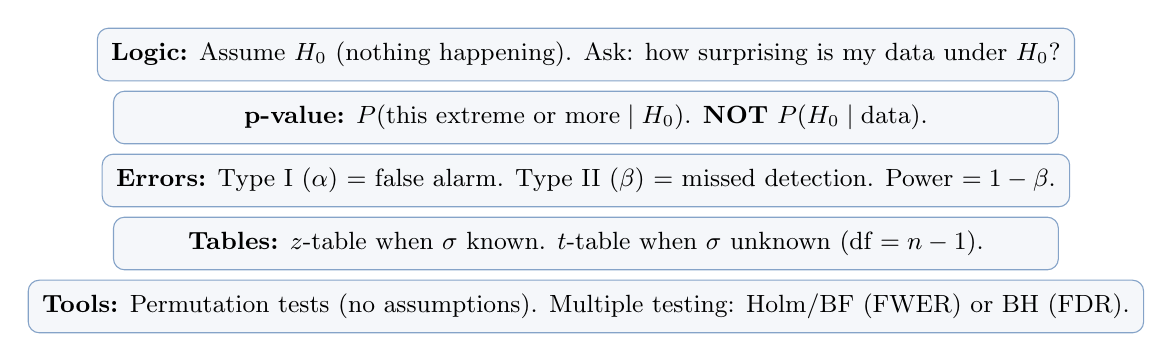
\begin{tikzpicture}[
  sbox/.style={draw=popblue!60, fill=popblue!5, rounded corners=4pt, minimum width=12cm, minimum height=0.5cm, align=left, inner sep=5pt, font=\small}
]
  \node[sbox] at (0, 2.0) {\textbf{Logic:} Assume $H_0$ (nothing happening). Ask: how surprising is my data under $H_0$?};
  \node[sbox] at (0, 1.2) {\textbf{p-value:} $P(\text{this extreme or more} \mid H_0)$. \textbf{NOT} $P(H_0 \mid \text{data})$.};
  \node[sbox] at (0, 0.4) {\textbf{Errors:} Type I ($\alpha$) = false alarm. Type II ($\beta$) = missed detection. Power $= 1 - \beta$.};
  \node[sbox] at (0, -0.4) {\textbf{Tables:} $z$-table when $\sigma$ known. $t$-table when $\sigma$ unknown (df $= n - 1$).};
  \node[sbox] at (0, -1.2) {\textbf{Tools:} Permutation tests (no assumptions). Multiple testing: Holm/BF (FWER) or BH (FDR).};
\end{tikzpicture}
\end{center}

\vspace{0.3cm}
\begin{center}
{\large\textbf{Today:}} The framework is clear. But which \textbf{specific test} do I actually use?
\end{center}
\end{frame}

% ============================================================
% NEW: TODAY'S PLAN
% ============================================================
\begin{frame}
\frametitle{Today's Plan: A Tour, Then a Unification}

\small
We'll meet the named tests one by one, like tools on a shelf. At the end, we'll pull back and see they're all the same machine.

\vspace{0.25cm}
\begin{center}
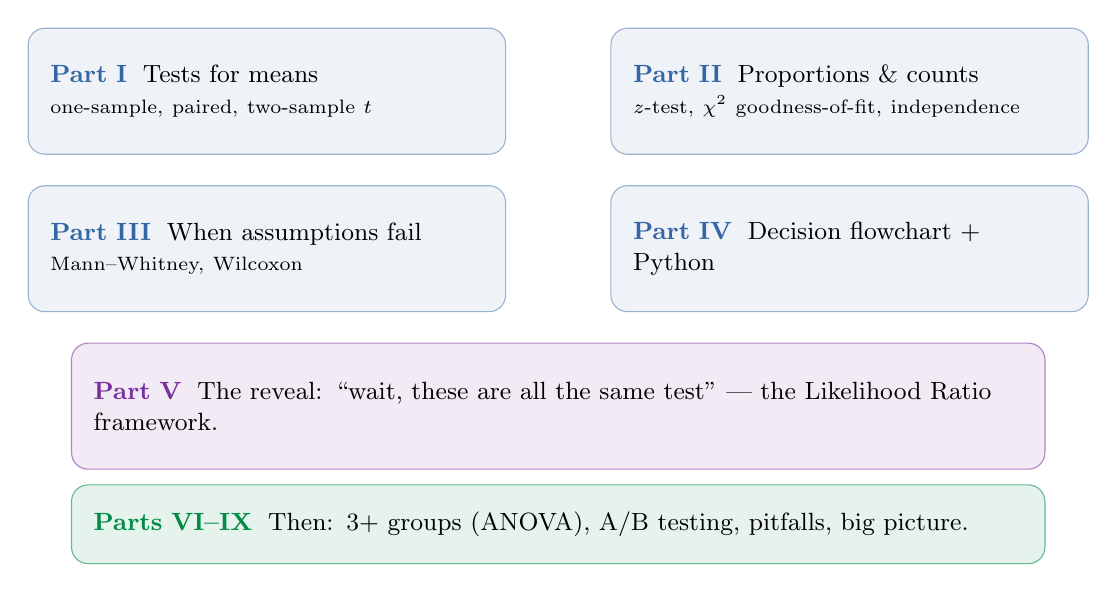
\begin{tikzpicture}[
  pbox/.style={draw, rounded corners=6pt, text width=5.5cm, align=left, inner sep=8pt, font=\small, minimum height=1.6cm}
]
  \node[pbox, fill=popblue!8, draw=popblue!50] at (-3.7, 2.2) {
    \textbf{\textcolor{popblue}{Part I}}\; Tests for means\\
    \scriptsize one-sample, paired, two-sample $t$
  };
  \node[pbox, fill=popblue!8, draw=popblue!50] at (3.7, 2.2) {
    \textbf{\textcolor{popblue}{Part II}}\; Proportions \& counts\\
    \scriptsize $z$-test, $\chi^2$ goodness-of-fit, independence
  };
  \node[pbox, fill=popblue!8, draw=popblue!50] at (-3.7, 0.2) {
    \textbf{\textcolor{popblue}{Part III}}\; When assumptions fail\\
    \scriptsize Mann--Whitney, Wilcoxon
  };
  \node[pbox, fill=popblue!8, draw=popblue!50] at (3.7, 0.2) {
    \textbf{\textcolor{popblue}{Part IV}}\; Decision flowchart + Python
  };
  \node[pbox, fill=violet1!10, draw=violet1!60, text width=11.8cm] at (0, -1.8) {
    \textbf{\textcolor{violet1}{Part V}}\; The reveal: ``wait, these are all the same test'' --- the Likelihood Ratio framework.
  };
  \node[pbox, fill=paramgreen!10, draw=paramgreen!60, text width=11.8cm, minimum height=1cm] at (0, -3.3) {
    \textbf{\textcolor{paramgreen}{Parts VI--IX}}\; Then: 3+ groups (ANOVA), A/B testing, pitfalls, big picture.
  };
\end{tikzpicture}
\end{center}
\end{frame}

% ============================================================
% PART I: TESTS FOR MEANS
% ============================================================
\section{Tests for Means}

\begin{frame}
\begin{center}
  \vspace{1.5cm}
  {\Huge\bfseries\textcolor{popblue}{Part I: Tests for Means}}

  \vspace{0.8cm}
  {\large One-sample, paired, two-sample}
\end{center}
\end{frame}

\begin{frame}
\frametitle{One-Sample $t$-Test}

\begin{center}
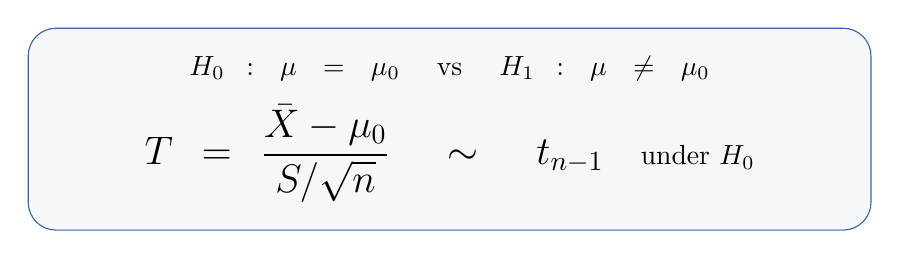
\begin{tikzpicture}
  \node[draw=popblue, fill=popblue!5, rounded corners=10pt, text width=10cm, align=center, inner sep=10pt] {
    $H_0\!: \mu = \mu_0$ \quad vs \quad $H_1\!: \mu \neq \mu_0$\\[8pt]
    {\Large $T = \dfrac{\bar{X} - \mu_0}{S / \sqrt{n}} \;\sim\; t_{n-1}$} \quad under $H_0$
  };
\end{tikzpicture}
\end{center}

\vspace{0.05cm}
\small
\textbf{Example:} Coffee shop claims cups contain $\mu_0 = 350$\,mL. We measure $n = 25$: $\bar{X} = 345$, $S = 10$.

\vspace{-0.2cm}
$$T = \frac{345 - 350}{10/\sqrt{25}} = \frac{-5}{2} = -2.50, \qquad p = 2 \cdot P(t_{24} < -2.50) \approx 0.020$$

\vspace{-0.1cm}
\begin{center}
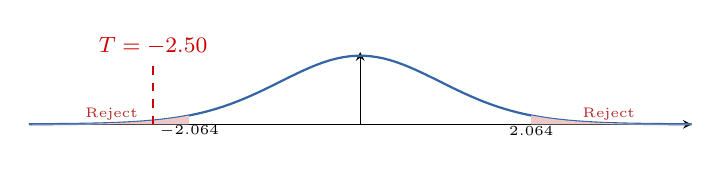
\begin{tikzpicture}
  \begin{axis}[
    width=10cm, height=2.5cm,
    domain=-4:4, samples=100,
    axis lines=middle, ticks=none,
    ymin=0, ymax=0.42,
    every axis plot/.style={thick, no markers},
    clip=false
  ]
    \addplot[popblue, thick] {(1 + x^2/24)^(-12.5) * 0.3989};
    \addplot[fill=warnred!25, draw=none, domain=-4:-2.064] {(1 + x^2/24)^(-12.5) * 0.3989} \closedcycle;
    \addplot[fill=warnred!25, draw=none, domain=2.064:4] {(1 + x^2/24)^(-12.5) * 0.3989} \closedcycle;
    \draw[thick, dashed, sampred] (axis cs:-2.50, 0) -- (axis cs:-2.50, 0.35);
    \node[font=\footnotesize\bfseries, sampred, above] at (axis cs:-2.50, 0.35) {$T = -2.50$};
    \node[font=\tiny, warnred] at (axis cs:-3, 0.06) {Reject};
    \node[font=\tiny, warnred] at (axis cs:3, 0.06) {Reject};
    \node[font=\tiny] at (axis cs:-2.064, -0.04) {$-2.064$};
    \node[font=\tiny] at (axis cs:2.064, -0.04) {$2.064$};
  \end{axis}
\end{tikzpicture}
\end{center}

\vspace{-0.05cm}
$p = 0.020 < 0.05$: \textbf{reject} $H_0$. The cups are underfilled.

\vspace{0.02cm}
{\scriptsize\textcolor{gray}{\textbf{Assumptions:} (1) Approx.\ Normal (or $n \geq 30$), (2) independent. Non-Normal + small $n$: Wilcoxon (Part~III). \;\textbf{One-sided:} $H_1\!: \mu > \mu_0$ or $\mu < \mu_0$ --- one tail only.}}
\end{frame}

\begin{frame}
\frametitle{Paired $t$-Test: Before vs After}

\small
If you have paired observations $(X_i, Y_i)$, compute differences $D_i = X_i - Y_i$ and apply a one-sample $t$-test on $D_i$.

\vspace{0.1cm}
\begin{center}
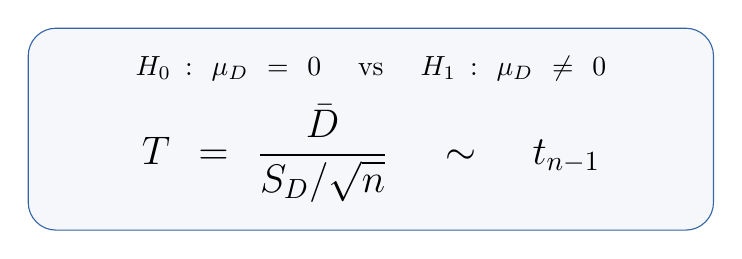
\begin{tikzpicture}
  \node[draw=popblue, fill=popblue!5, rounded corners=10pt, text width=8cm, align=center, inner sep=10pt] {
    $H_0\!: \mu_D = 0$ \quad vs \quad $H_1\!: \mu_D \neq 0$\\[8pt]
    {\Large $T = \dfrac{\bar{D}}{S_D / \sqrt{n}} \;\sim\; t_{n-1}$}
  };
\end{tikzpicture}
\end{center}

\vspace{0.1cm}
\textbf{Example:} Blood pressure before/after drug, $n = 8$ patients.

\vspace{0.1cm}
\begin{center}
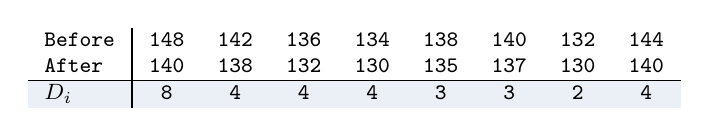
\begin{tikzpicture}
  \node[font=\footnotesize\ttfamily, inner sep=0pt] {
    \begin{tabular}{l|cccccccc}
      Before & 148 & 142 & 136 & 134 & 138 & 140 & 132 & 144 \\
      After  & 140 & 138 & 132 & 130 & 135 & 137 & 130 & 140 \\
      \hline
      \rowcolor{popblue!10}
      $D_i$  & 8 & 4 & 4 & 4 & 3 & 3 & 2 & 4 \\
    \end{tabular}
  };
\end{tikzpicture}
\end{center}

\vspace{0.1cm}
$\bar{D} = 4.0$, \;$S_D = 1.77$, \;$T = \dfrac{4.0}{1.77/\sqrt{8}} = 6.39$, \;$p \approx 0.0004$.

\vspace{0.05cm}
$p \ll 0.05$: \textbf{reject} $H_0$. The drug works. \; Cohen's $d = \bar{D}/S_D = 4.0/1.77 = 2.26$ (very large).
\end{frame}

\begin{frame}
\frametitle{Why Pairing Matters: Same Data, Two Stories}
\framesubtitle{Run the BP example as if it were unpaired --- watch the verdict change}

\small
The paired analysis on the previous slide gave $T = 6.39$, $p \approx 0.0004$.\\
What if we (wrongly) treat ``before'' and ``after'' as two independent groups?

\vspace{0.15cm}
\begin{center}
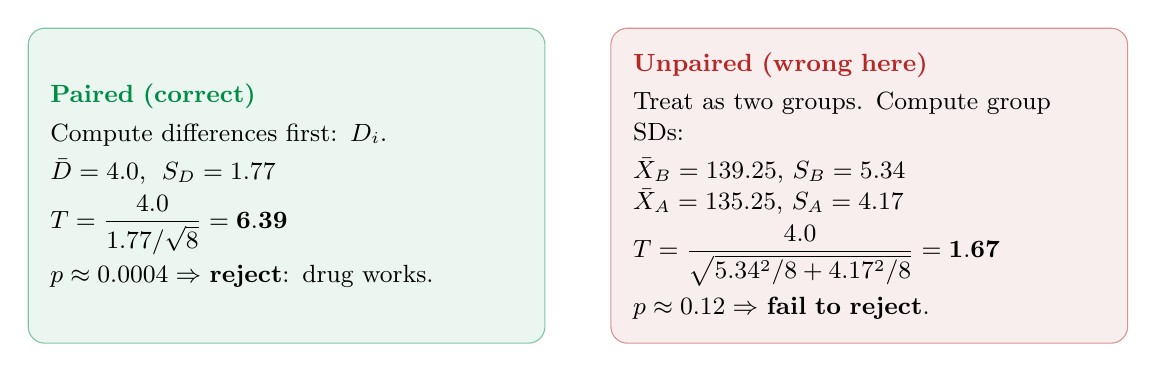
\begin{tikzpicture}[
  cbox/.style={draw, rounded corners=6pt, text width=6cm, align=left, inner sep=8pt, font=\small, minimum height=4.0cm}
]
  \node[cbox, fill=paramgreen!8, draw=paramgreen!50] at (-3.7, 0) {
    \textbf{\textcolor{paramgreen}{Paired (correct)}}\\[3pt]
    Compute differences first: $D_i$.\\[3pt]
    $\bar D = 4.0$, \;$S_D = 1.77$\\[3pt]
    $T = \dfrac{4.0}{1.77/\sqrt{8}} = \mathbf{6.39}$\\[3pt]
    $p \approx 0.0004 \Rightarrow$ \textbf{reject}: drug works.
  };
  \node[cbox, fill=warnred!8, draw=warnred!50] at (3.7, 0) {
    \textbf{\textcolor{warnred}{Unpaired (wrong here)}}\\[3pt]
    Treat as two groups. Compute group SDs:\\[3pt]
    $\bar X_B = 139.25$, $S_B = 5.34$\\
    $\bar X_A = 135.25$, $S_A = 4.17$\\[3pt]
    $T = \dfrac{4.0}{\sqrt{5.34^2/8 + 4.17^2/8}} = \mathbf{1.67}$\\[3pt]
    $p \approx 0.12 \Rightarrow$ \textbf{fail to reject}.
  };
\end{tikzpicture}
\end{center}

\vspace{0.1cm}
\begin{center}
\fcolorbox{popblue}{popblue!5}{\parbox{12cm}{\centering\footnotesize
  \textbf{Why so different?}\; The patient-to-patient BP swing ($\sim 16$ mmHg, hence $S_B \approx 5$) dominates the drug effect ($\sim 4$ mmHg). Unpaired treats that swing as ``noise''. Paired \emph{cancels it out}: each patient is their own baseline, leaving only the within-patient change ($S_D = 1.77$, roughly $3\times$ smaller SD, $\sim 9\times$ less variance).
}}
\end{center}
\end{frame}

\begin{frame}
\frametitle{Two-Sample $t$-Test (Welch's): Comparing Two Groups}
\framesubtitle{Two independent groups, $(\bar X_1, S_1, n_1)$ and $(\bar X_2, S_2, n_2)$}

\small
\textbf{Building the statistic:} the numerator is the observed difference of means $\bar X_1 - \bar X_2$. The denominator is its standard error.

\vspace{0.1cm}
\begin{center}
\fcolorbox{popblue}{popblue!5}{\parbox{12cm}{\small
  Since the samples are \emph{independent}: $\;\text{Var}(\bar X_1 - \bar X_2) = \text{Var}(\bar X_1) + \text{Var}(\bar X_2) = \sigma_1^2/n_1 + \sigma_2^2/n_2$. \;Plug in $S_i^2$ for $\sigma_i^2$:
}}
\end{center}

\vspace{0.05cm}
\begin{center}
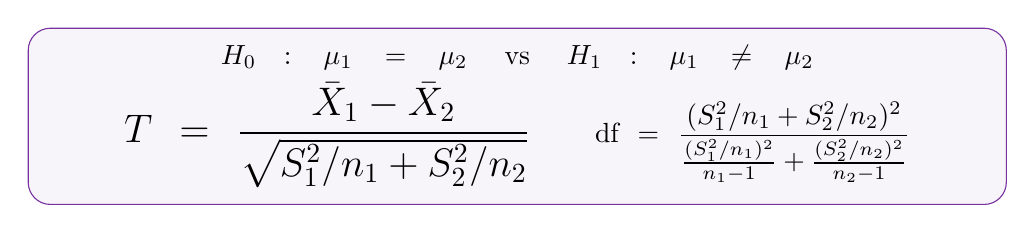
\begin{tikzpicture}
  \node[draw=violet1, fill=violet1!5, rounded corners=8pt, text width=12cm, align=center, inner sep=6pt] {
    $H_0\!: \mu_1 = \mu_2$ \quad vs \quad $H_1\!: \mu_1 \neq \mu_2$\\[4pt]
    {\Large $T = \dfrac{\bar{X}_1 - \bar{X}_2}{\sqrt{S_1^2/n_1 + S_2^2/n_2}}$} \qquad
    $\text{df} = \dfrac{(S_1^2/n_1 + S_2^2/n_2)^2}{\frac{(S_1^2/n_1)^2}{n_1-1} + \frac{(S_2^2/n_2)^2}{n_2-1}}$
  };
\end{tikzpicture}
\end{center}

\vspace{0.05cm}
\textbf{Why the awkward df?} It's a weighted average of $n_1{-}1$ and $n_2{-}1$ that adjusts for the two unequal variance estimates. Usually a non-integer; \texttt{scipy} rounds and uses tables.

\vspace{0.05cm}
\begin{center}
\fcolorbox{orange1}{orange1!5}{\parbox{11.5cm}{\centering\footnotesize
  \textbf{Default to Welch's.} R and Python use it by default. The pooled $t$-test assumes $\sigma_1 = \sigma_2$; tiny extra power, not worth the assumption.
}}
\end{center}
\end{frame}

\begin{frame}
\frametitle{Two-Sample Worked Example: Two Teaching Methods}

\small
Method A ($n_1 = 10$): $\bar{X}_1 = 82.3$, $S_1 = 8.5$. \quad
Method B ($n_2 = 12$): $\bar{X}_2 = 74.1$, $S_2 = 10.2$.

\vspace{0.1cm}
\textbf{Welch's $t$-test:}
$$T = \frac{82.3 - 74.1}{\sqrt{8.5^2/10 + 10.2^2/12}} = \frac{8.2}{\sqrt{7.225 + 8.67}} = \frac{8.2}{3.99} = 2.06$$

$\text{df} \approx 19.8$, \;$t_{19.8,\, 0.025} \approx 2.09$, \;$p \approx 0.053$.

\vspace{0.1cm}
\begin{center}
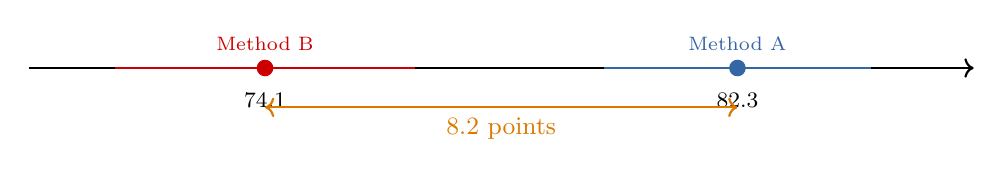
\begin{tikzpicture}
  \draw[thick, ->] (0, 0) -- (12, 0);
  \node[font=\footnotesize, below] at (3, -0.2) {74.1};
  \node[font=\footnotesize, below] at (9, -0.2) {82.3};
  \draw[thick, popblue] (9, -0.05) -- (9, 0.05);
  \fill[popblue] (9, 0) circle (3pt);
  \draw[thick, popblue] (7.3, 0) -- (10.7, 0);
  \node[font=\scriptsize, popblue, above] at (9, 0.1) {Method A};
  \draw[thick, sampred] (3, -0.05) -- (3, 0.05);
  \fill[sampred] (3, 0) circle (3pt);
  \draw[thick, sampred] (1.1, 0) -- (4.9, 0);
  \node[font=\scriptsize, sampred, above] at (3, 0.1) {Method B};
  \draw[<->, thick, orange1] (3, -0.5) -- (9, -0.5) node[midway, below, font=\small] {$8.2$ points};
\end{tikzpicture}
\end{center}

\vspace{0.05cm}
$|T| = 2.06 < 2.09$: \textbf{fail to reject} at $\alpha = 0.05$ (just barely!).
Cohen's $d \approx 0.87$ (large effect) --- the data \emph{look} like a real gap, but $n$ is too small to call it. Underpowered, not no-effect.
\end{frame}

% ============================================================
% PART II: PROPORTIONS AND COUNTS
% ============================================================
\section{Proportions and Counts}

\begin{frame}
\begin{center}
  \vspace{1.5cm}
  {\Huge\bfseries\textcolor{popblue}{Part II: Proportions and Counts}}

  \vspace{0.8cm}
  {\large $z$-test for one proportion, $\chi^2$ for tables of counts}
\end{center}
\end{frame}

\begin{frame}
\frametitle{Test for a Proportion}

\begin{center}
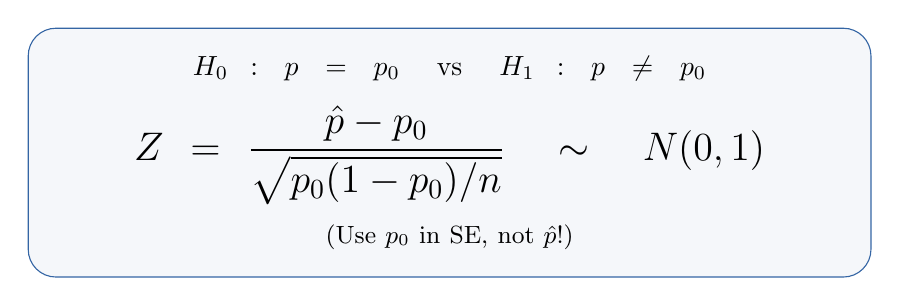
\begin{tikzpicture}
  \node[draw=popblue, fill=popblue!5, rounded corners=10pt, text width=10cm, align=center, inner sep=10pt] {
    $H_0\!: p = p_0$ \quad vs \quad $H_1\!: p \neq p_0$\\[8pt]
    {\Large $Z = \dfrac{\hat{p} - p_0}{\sqrt{p_0(1-p_0)/n}} \;\sim\; N(0,1)$}\\[6pt]
    \small (Use $p_0$ in SE, not $\hat{p}$!)
  };
\end{tikzpicture}
\end{center}

\vspace{0.15cm}
\small
\textbf{Example:} Is a coin fair? $n = 200$ flips, $k = 115$ heads, $\hat{p} = 0.575$.

$$Z = \frac{0.575 - 0.5}{\sqrt{0.5 \times 0.5/200}} = \frac{0.075}{0.0354} = 2.12, \qquad p = 2(1 - \Phi(2.12)) = 0.034$$

$p < 0.05$: \textbf{reject} $H_0$. Evidence the coin is biased.

\vspace{0.15cm}
\begin{center}
\fcolorbox{orange1}{orange1!5}{\parbox{10cm}{\centering\small
  \textbf{Rule of thumb:} use this test when $np_0 \geq 10$ and $n(1 - p_0) \geq 10$.\\
  For two proportions: $Z = \frac{\hat{p}_1 - \hat{p}_2}{\sqrt{\hat{p}(1-\hat{p})(1/n_1 + 1/n_2)}}$
  where $\hat{p} = \frac{k_1 + k_2}{n_1 + n_2}$ (pooled under $H_0\!: p_1 = p_2$).
}}
\end{center}
\end{frame}

% --- NEW: motivation transition slide ---
\begin{frame}
\frametitle{What About Many Categories?}
\framesubtitle{The $z$-test handled 2 outcomes. What about 6 (a die) or a $2 \times 3$ table?}

\small
For each of $k$ categories we have an \textbf{observed} count $O_i$ and an \textbf{expected} count $E_i$ (under $H_0$). We want one number that summarises ``how off'' the data are.

\vspace{0.15cm}
\begin{center}
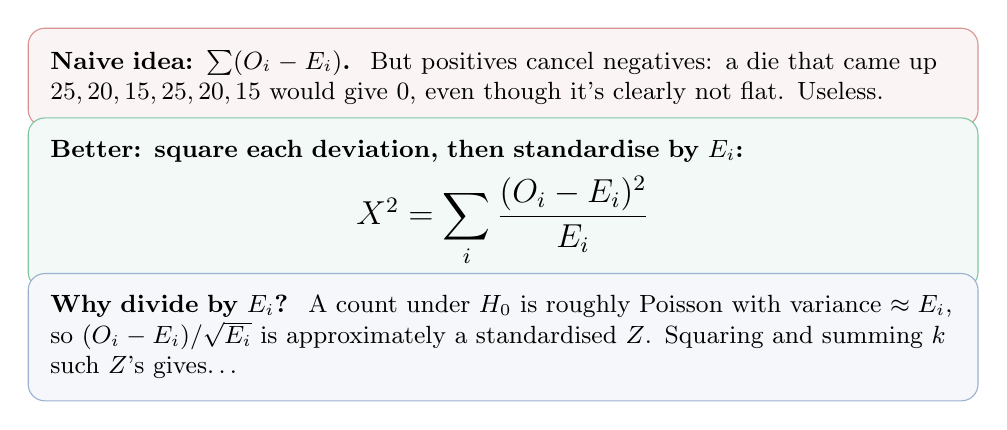
\begin{tikzpicture}[
  obox/.style={draw, rounded corners=6pt, text width=11.5cm, align=left, inner sep=8pt, font=\small}
]
  \node[obox, fill=warnred!5, draw=warnred!50] at (0, 1.6) {
    \textbf{Naive idea: $\sum (O_i - E_i)$.}\; But positives cancel negatives: a die that came up $25, 20, 15, 25, 20, 15$ would give $0$, even though it's clearly not flat. Useless.
  };
  \node[obox, fill=paramgreen!5, draw=paramgreen!50] at (0, 0.0) {
    \textbf{Better: square each deviation, then standardise by $E_i$:}\\[4pt]
    \centerline{\large $X^2 = \displaystyle\sum_i \frac{(O_i - E_i)^2}{E_i}$}
  };
  \node[obox, fill=popblue!5, draw=popblue!50] at (0, -1.7) {
    \textbf{Why divide by $E_i$?}\; A count under $H_0$ is roughly Poisson with variance $\approx E_i$, so $(O_i - E_i)/\sqrt{E_i}$ is approximately a standardised $Z$. Squaring and summing $k$ such $Z$'s gives\ldots
  };
\end{tikzpicture}
\end{center}

\vspace{0.05cm}
\begin{center}
{\large \ldots a \textbf{$\chi^2$ distribution.} (Defined on the next slide.)}
\end{center}
\end{frame}

% --- chi-squared distribution intro ---
\begin{frame}
\frametitle{The $\chi^2$ Distribution}
\framesubtitle{Sum of squared independent standard normals}

\small
\textbf{Definition:} if $Z_1, \ldots, Z_k$ are independent $N(0,1)$, then
$$Z_1^2 + Z_2^2 + \cdots + Z_k^2 \;\sim\; \chi^2_k \quad \text{(``chi-squared with $k$ degrees of freedom'')}.$$

\vspace{0.05cm}
\begin{center}
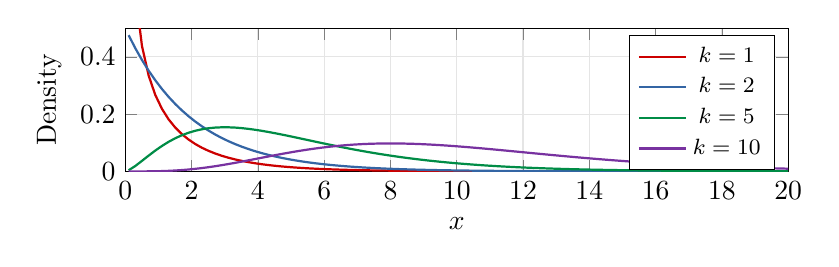
\begin{tikzpicture}
  \begin{axis}[
    width=10cm, height=3.4cm,
    domain=0.1:20, samples=100,
    xlabel={$x$}, ylabel={Density},
    xmin=0, xmax=20, ymin=0, ymax=0.5,
    grid=major, grid style={gray!20},
    legend style={at={(0.98,0.95)}, anchor=north east, font=\footnotesize},
    every axis plot/.style={thick, no markers}
  ]
    \addplot[sampred] {x^(-0.5) * exp(-x/2) / (sqrt(2*pi))};
    \addlegendentry{$k = 1$}
    \addplot[popblue] {0.5 * exp(-x/2)};
    \addlegendentry{$k = 2$}
    \addplot[paramgreen] {x^(1.5) * exp(-x/2) / (5.657 * 1.3293)};
    \addlegendentry{$k = 5$}
    \addplot[violet1] {x^(4) * exp(-x/2) / (32 * 24)};
    \addlegendentry{$k = 10$}
  \end{axis}
\end{tikzpicture}
\end{center}

\vspace{0.05cm}
\begin{center}
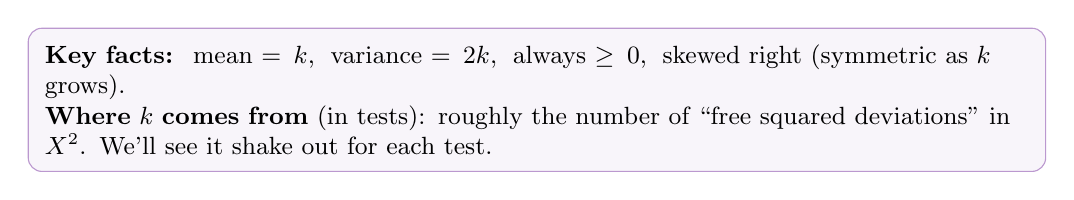
\begin{tikzpicture}
  \node[draw=violet1!50, fill=violet1!5, rounded corners=5pt, text width=12.5cm, align=left, inner sep=6pt, font=\small] {
    \textbf{Key facts:}\; mean $= k$, \;variance $= 2k$, \;always $\geq 0$, \;skewed right (symmetric as $k$ grows).\\
    \textbf{Where $k$ comes from} (in tests): roughly the number of ``free squared deviations'' in $X^2$. We'll see it shake out for each test.
  };
\end{tikzpicture}
\end{center}
\end{frame}

\begin{frame}
\frametitle{Goodness-of-Fit: Is a Die Loaded?}

\small
\textbf{Story:} Someone hands you a die. You suspect it's loaded. You roll it $n = 120$ times.

\vspace{0.05cm}
\begin{center}
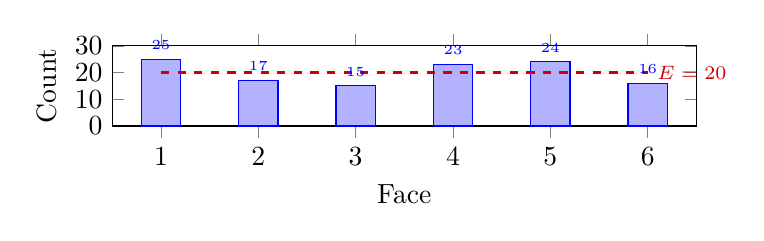
\begin{tikzpicture}
  \begin{axis}[
    width=9cm, height=2.6cm,
    ybar,
    bar width=0.5cm,
    xlabel={Face}, ylabel={Count},
    symbolic x coords={1,2,3,4,5,6},
    xtick=data,
    ymin=0, ymax=30,
    nodes near coords,
    nodes near coords style={font=\tiny},
    every axis plot/.style={fill=popblue!50, draw=popblue!70},
    clip=false
  ]
    \addplot coordinates {(1,25) (2,17) (3,15) (4,23) (5,24) (6,16)};
    \draw[thick, dashed, sampred] (axis cs:1, 20) -- (axis cs:6, 20);
    \node[font=\scriptsize, sampred, right] at (axis cs:6, 20) {$E = 20$};
  \end{axis}
\end{tikzpicture}
\end{center}

\vspace{-0.05cm}
\textbf{Question:} could a fair die have produced this much wobble around the expected $20$ per face?

\vspace{0.1cm}
\begin{center}
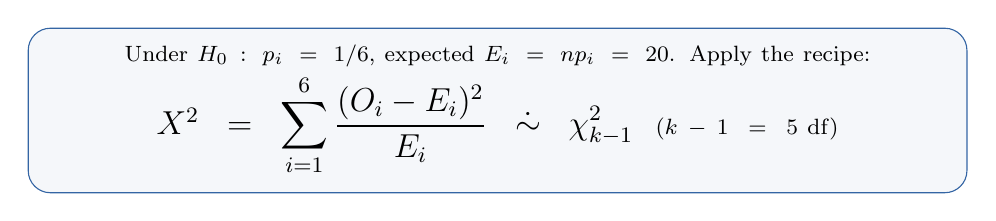
\begin{tikzpicture}
  \node[draw=popblue, fill=popblue!5, rounded corners=8pt, text width=11.5cm, align=center, inner sep=6pt] {
    \footnotesize Under $H_0\!: p_i = 1/6$, expected $E_i = n p_i = 20$. Apply the recipe:\\[2pt]
    {\large $X^2 = \displaystyle\sum_{i=1}^{6} \frac{(O_i - E_i)^2}{E_i} \;\dot{\sim}\; \chi^2_{k-1}$} \;\;($k - 1 = 5$ df)
  };
\end{tikzpicture}
\end{center}

\vspace{0.02cm}
\small
$X^2 = \frac{25 + 9 + 25 + 9 + 16 + 16}{20} = 5.0$. \;\;Critical: $\chi^2_{5,\,0.05} = 11.07$. \;\;$5.0 < 11.07$: \textbf{fail to reject}. The wobble is consistent with chance --- no evidence the die is loaded.

\vspace{0.02cm}
{\scriptsize\textcolor{gray}{\textbf{Why $k - 1$, not $k$?} The six counts sum to $n$, so once five are known the sixth is fixed. Only $5$ are free to deviate.}}
\end{frame}

\begin{frame}
\frametitle{Test of Independence: Two Categorical Variables}

\small
\textbf{Setup:} Contingency table with $r$ rows and $c$ columns. $H_0$: variables are independent.

\vspace{0.1cm}
\begin{center}
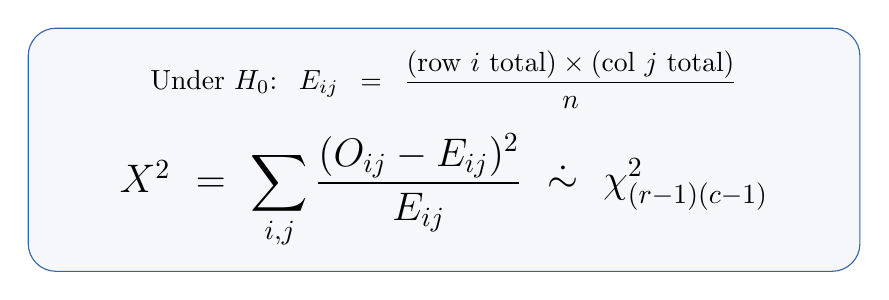
\begin{tikzpicture}
  \node[draw=popblue, fill=popblue!5, rounded corners=10pt, text width=10cm, align=center, inner sep=8pt] {
    Under $H_0$:\; $E_{ij} = \dfrac{(\text{row } i \text{ total}) \times (\text{col } j \text{ total})}{n}$\\[8pt]
    {\Large $X^2 = \displaystyle\sum_{i,j} \frac{(O_{ij} - E_{ij})^2}{E_{ij}} \;\dot{\sim}\; \chi^2_{(r-1)(c-1)}$}
  };
\end{tikzpicture}
\end{center}

\pause
\vspace{0.1cm}
\textbf{Example: Smoking and lung cancer} ($n = 200$).

\vspace{0.05cm}
\begin{center}
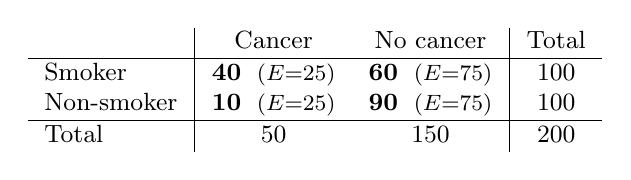
\begin{tikzpicture}
  \node[font=\small, inner sep=0pt] {
    \begin{tabular}{l|cc|c}
      & Cancer & No cancer & Total \\
      \hline
      Smoker & \textbf{40} \;\footnotesize{($E{=}25$)} & \textbf{60} \;\footnotesize{($E{=}75$)} & 100 \\
      Non-smoker & \textbf{10} \;\footnotesize{($E{=}25$)} & \textbf{90} \;\footnotesize{($E{=}75$)} & 100 \\
      \hline
      Total & 50 & 150 & 200 \\
    \end{tabular}
  };
\end{tikzpicture}
\end{center}

\vspace{0.02cm}
$X^2 = \frac{(40{-}25)^2}{25} + \frac{(60{-}75)^2}{75} + \frac{(10{-}25)^2}{25} + \frac{(90{-}75)^2}{75} = 9 + 3 + 9 + 3 = \mathbf{24.0}$

\vspace{0.05cm}
df $= (2{-}1)(2{-}1) = 1$. \;$\chi^2_{1,\,0.05} = 3.84$. \;$24.0 \gg 3.84$: \textbf{reject}. Strong association.

\vspace{0.02cm}
{\scriptsize\textcolor{gray}{\textbf{$\chi^2$ detects \emph{association}, not \emph{causation}} --- could be a hidden confounder (see L14).}}
\end{frame}

% ============================================================
% PART III: NONPARAMETRIC ALTERNATIVES
% ============================================================
\section{When Assumptions Fail}

\begin{frame}
\begin{center}
  \vspace{1.5cm}
  {\Huge\bfseries\textcolor{popblue}{Part III: When Assumptions Fail}}

  \vspace{0.8cm}
  {\large Nonparametric alternatives: no Normal required}
\end{center}
\end{frame}

\begin{frame}
\frametitle{Mann--Whitney $U$ Test}
\framesubtitle{Comparing two independent groups --- nonparametric alternative to two-sample $t$}

\small
\textbf{Use case:} you A/B-test two checkout flows and record \textit{completion time}. Most users finish in $\sim 30$\,s, but a few hit the bathroom mid-flow and take 20 minutes. A $t$-test gets dragged around by those outliers; the means become useless. \textbf{Mann--Whitney} replaces every value with its \emph{rank} --- the slow outlier becomes ``last,'' nothing more.

\vspace{0.15cm}
\textbf{Idea:} pool all values, rank them $1, 2, \ldots, n_1 + n_2$, sum each group's ranks.

\vspace{0.1cm}
\begin{center}
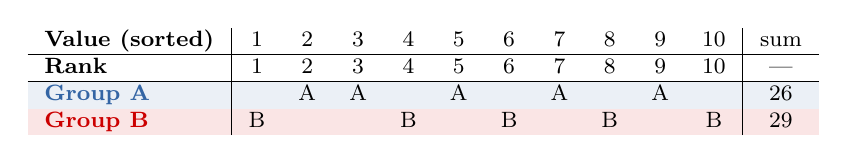
\begin{tikzpicture}
  \node[font=\footnotesize, inner sep=0pt] {
    \begin{tabular}{l|cccccccccc|c}
      \textbf{Value (sorted)} &  1 &  2 &  3 &  4 &  5 &  6 &  7 &  8 &  9 & 10 & sum \\
      \hline
      \textbf{Rank}           &  1 &  2 &  3 &  4 &  5 &  6 &  7 &  8 &  9 & 10 & --- \\
      \hline
      \rowcolor{popblue!10}
      \textbf{\textcolor{popblue}{Group A}}        &    & A  & A  &    & A  &    & A  &    & A  &    & 26 \\
      \rowcolor{sampred!10}
      \textbf{\textcolor{sampred}{Group B}}        & B  &    &    & B  &    & B  &    & B  &    & B  & 29 \\
    \end{tabular}
  };
\end{tikzpicture}
\end{center}

\vspace{0.15cm}
\begin{center}
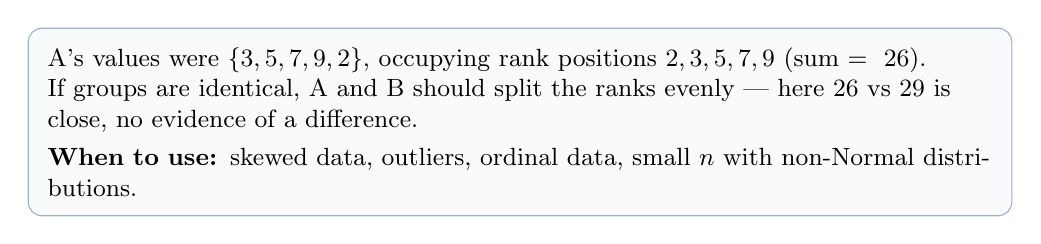
\begin{tikzpicture}
  \node[draw=popblue!50, fill=popblue!3, rounded corners=5pt, text width=12cm, align=left, inner sep=7pt, font=\small] {
    A's values were $\{3, 5, 7, 9, 2\}$, occupying rank positions $2, 3, 5, 7, 9$ (sum $= 26$). If groups are identical, A and B should split the ranks evenly --- here $26$ vs $29$ is close, no evidence of a difference.\\[3pt]
    \textbf{When to use:} skewed data, outliers, ordinal data, small $n$ with non-Normal distributions.
  };
\end{tikzpicture}
\end{center}
\end{frame}

\begin{frame}
\frametitle{Wilcoxon Signed-Rank Test (1/2): The Idea}
\framesubtitle{Paired nonparametric alternative to the paired $t$-test}

\small
\textbf{Setup:} same as paired $t$ --- $n$ paired observations, compute differences $D_i$. Difference: instead of using $\bar D$ and $S_D$, we use \emph{ranks} of $|D_i|$.

\vspace{0.15cm}
\begin{center}
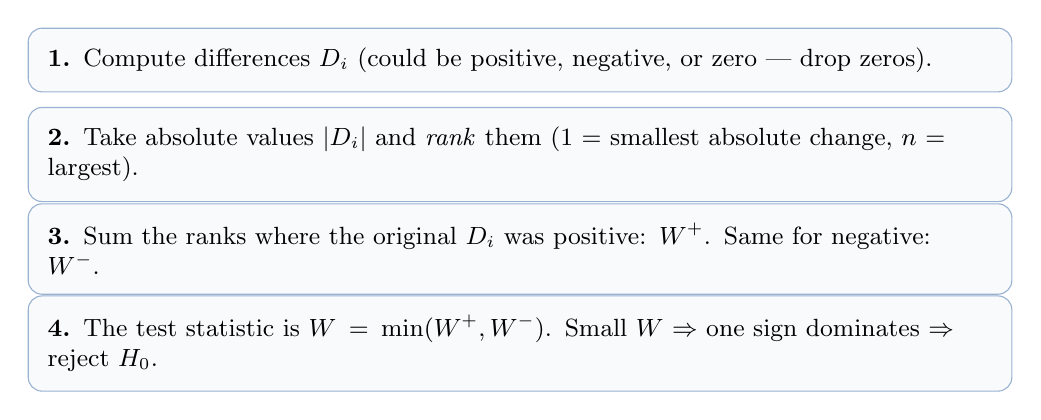
\begin{tikzpicture}[
  wstep/.style={draw=popblue!50, fill=popblue!3, rounded corners=5pt, text width=12cm, align=left, inner sep=7pt, font=\small}
]
  \node[wstep] at (0, 1.6) {
    \textbf{1.} Compute differences $D_i$ (could be positive, negative, or zero --- drop zeros).
  };
  \node[wstep] at (0, 0.4) {
    \textbf{2.} Take absolute values $|D_i|$ and \emph{rank} them ($1$ = smallest absolute change, $n$ = largest).
  };
  \node[wstep] at (0, -0.8) {
    \textbf{3.} Sum the ranks where the original $D_i$ was positive: $W^+$. Same for negative: $W^-$.
  };
  \node[wstep] at (0, -2.0) {
    \textbf{4.} The test statistic is $W = \min(W^+, W^-)$. Small $W$ $\Rightarrow$ one sign dominates $\Rightarrow$ reject $H_0$.
  };
\end{tikzpicture}
\end{center}

\vspace{0.15cm}
\begin{center}
\fcolorbox{popblue}{popblue!5}{\parbox{11cm}{\centering\footnotesize
  \textbf{Intuition:} if the treatment has no effect, half the differences should be positive, half negative, with similar magnitudes. So the rank sums should split roughly evenly.
}}
\end{center}
\end{frame}

\begin{frame}
\frametitle{Wilcoxon Signed-Rank Test (2/2): Worked Example}

\small
\textbf{Data:} 7 students, scores before vs after a workshop. Mostly improved, two slipped.

\vspace{0.15cm}
\begin{center}
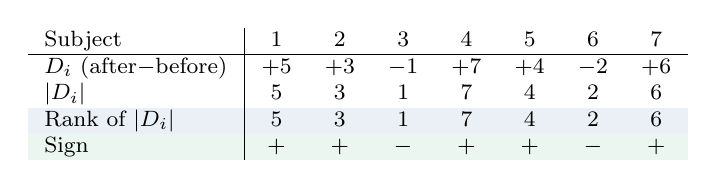
\begin{tikzpicture}
  \node[font=\footnotesize, inner sep=0pt] {
    \begin{tabular}{l|ccccccc}
      Subject              & 1 & 2 & 3 & 4 & 5 & 6 & 7 \\
      \hline
      $D_i$ (after$-$before)& $+5$ & $+3$ & $-1$ & $+7$ & $+4$ & $-2$ & $+6$ \\
      $|D_i|$              & 5 & 3 & 1 & 7 & 4 & 2 & 6 \\
      \rowcolor{popblue!10}
      Rank of $|D_i|$      & 5 & 3 & 1 & 7 & 4 & 2 & 6 \\
      \rowcolor{paramgreen!8}
      Sign                 & $+$ & $+$ & $-$ & $+$ & $+$ & $-$ & $+$ \\
    \end{tabular}
  };
\end{tikzpicture}
\end{center}

\vspace{0.1cm}
\textbf{Compute:} \quad $W^+ = 5 + 3 + 7 + 4 + 6 = 25$, \quad $W^- = 1 + 2 = 3$, \quad $W = \min(25, 3) = 3$.

\vspace{0.05cm}
\textbf{Decide:} at $n = 7$, two-sided $\alpha = 0.05$ rejects when $W \leq 2$. Here $W = 3$: \textbf{fail to reject} ($p \approx 0.063$ via normal approximation). Suggestive but not conclusive.

\vspace{0.15cm}
\begin{center}
\fcolorbox{orange1}{orange1!5}{\parbox{11.5cm}{\centering\footnotesize
  \textbf{When to use:} paired data that's not Normal; ordinal scales (e.g.\ Likert 1--5); small samples with outliers.\\
  \textbf{Trade-off:} $\sim 5\%$ less power than paired $t$ when data \emph{is} Normal --- a small price for safety.\\
  \textbf{Three or more groups, non-Normal:} Kruskal--Wallis (covered later).
}}
\end{center}
\end{frame}

% ============================================================
% PART IV: PUTTING IT TOGETHER
% ============================================================
\section{Putting It Together}

\begin{frame}
\begin{center}
  \vspace{1.5cm}
  {\Huge\bfseries\textcolor{popblue}{Part IV: Putting It Together}}

  \vspace{0.8cm}
  {\large Decision flowchart and Python}
\end{center}
\end{frame}

\begin{frame}
\frametitle{Which Test Do I Use?}

\begin{center}
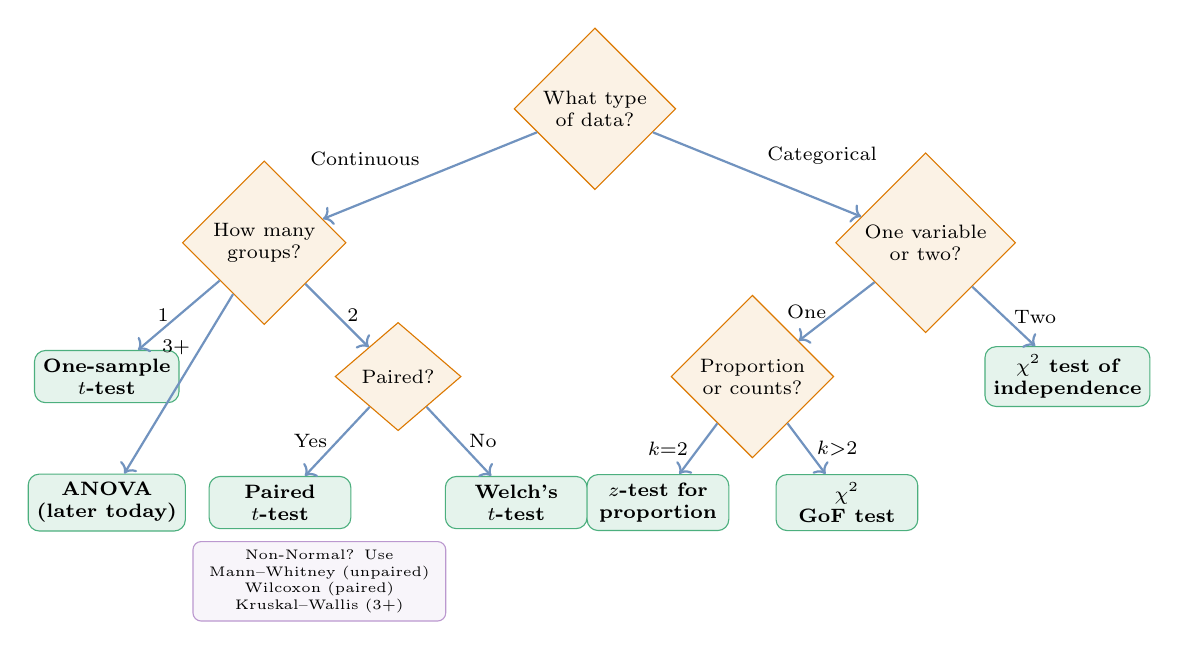
\begin{tikzpicture}[
  decision/.style={diamond, draw=orange1, fill=orange1!10, inner sep=2pt, font=\scriptsize, align=center, minimum width=1.6cm, minimum height=0.8cm},
  test/.style={rectangle, draw=paramgreen!70, fill=paramgreen!10, rounded corners=4pt, inner sep=3pt, font=\scriptsize\bfseries, align=center, minimum width=1.8cm},
  arr/.style={->, thick, draw=popblue!70},
  every node/.style={font=\scriptsize}
]
  \node[decision] (start) at (0, 3.2) {What type\\of data?};
  \node[decision] (ngroups) at (-4.2, 1.5) {How many\\groups?};
  \draw[arr] (start) -- node[above left] {Continuous} (ngroups);
  \node[test] (onet) at (-6.2, -0.2) {One-sample\\$t$-test};
  \draw[arr] (ngroups) -- node[left] {1} (onet);
  \node[decision] (paired) at (-2.5, -0.2) {Paired?};
  \draw[arr] (ngroups) -- node[right] {2} (paired);
  \node[test] (pairedt) at (-4, -1.8) {Paired\\$t$-test};
  \node[test] (welch) at (-1, -1.8) {Welch's\\$t$-test};
  \draw[arr] (paired) -- node[left] {Yes} (pairedt);
  \draw[arr] (paired) -- node[right] {No} (welch);
  \node[decision] (cattype) at (4.2, 1.5) {One variable\\or two?};
  \draw[arr] (start) -- node[above right] {Categorical} (cattype);
  \node[decision] (propn) at (2, -0.2) {Proportion\\or counts?};
  \draw[arr] (cattype) -- node[left] {One} (propn);
  \node[test] (zp) at (0.8, -1.8) {$z$-test for\\proportion};
  \node[test] (gof) at (3.2, -1.8) {$\chi^2$\\GoF test};
  \draw[arr] (propn) -- node[left] {$k{=}2$} (zp);
  \draw[arr] (propn) -- node[right] {$k{>}2$} (gof);
  \node[test] (indep) at (6, -0.2) {$\chi^2$ test of\\independence};
  \draw[arr] (cattype) -- node[right] {Two} (indep);
  \node[test] (anova) at (-6.2, -1.8) {ANOVA\\(later today)};
  \draw[arr] (ngroups) -- node[left, pos=0.3] {$3{+}$} (anova);
  \node[draw=violet1!50, fill=violet1!5, rounded corners=3pt, font=\tiny, text width=3cm, align=center, inner sep=3pt] at (-3.5, -2.8) {Non-Normal? Use\\Mann--Whitney (unpaired)\\Wilcoxon (paired)\\Kruskal--Wallis ($3{+}$)};
\end{tikzpicture}
\end{center}
\end{frame}

% --- NEW: scenarios table ---
\begin{frame}
\frametitle{Scenario Cheat Sheet}
\framesubtitle{Real-world question $\to$ test}

\footnotesize
\begin{center}
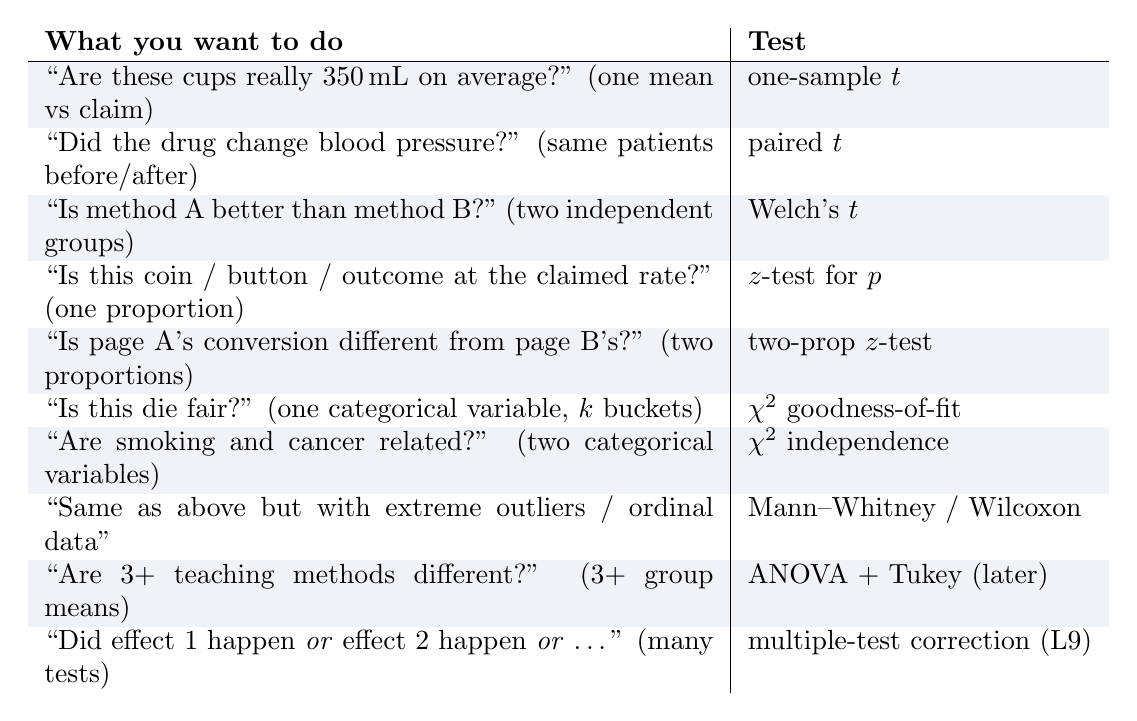
\begin{tikzpicture}
  \node[inner sep=0pt] {
    \begin{tabular}{p{8.5cm}|l}
      \textbf{What you want to do} & \textbf{Test} \\
      \hline
      \rowcolor{popblue!8}
      ``Are these cups really 350\,mL on average?'' (one mean vs claim) & one-sample $t$ \\
      ``Did the drug change blood pressure?'' (same patients before/after) & paired $t$ \\
      \rowcolor{popblue!8}
      ``Is method A better than method B?'' (two independent groups) & Welch's $t$ \\
      ``Is this coin / button / outcome at the claimed rate?'' (one proportion) & $z$-test for $p$ \\
      \rowcolor{popblue!8}
      ``Is page A's conversion different from page B's?'' (two proportions) & two-prop $z$-test \\
      ``Is this die fair?'' (one categorical variable, $k$ buckets) & $\chi^2$ goodness-of-fit \\
      \rowcolor{popblue!8}
      ``Are smoking and cancer related?'' (two categorical variables) & $\chi^2$ independence \\
      ``Same as above but with extreme outliers / ordinal data'' & Mann--Whitney / Wilcoxon \\
      \rowcolor{popblue!8}
      ``Are 3+ teaching methods different?'' (3+ group means) & ANOVA + Tukey (later) \\
      ``Did effect 1 happen \emph{or} effect 2 happen \emph{or} \ldots'' (many tests) & multiple-test correction (L9) \\
    \end{tabular}
  };
\end{tikzpicture}
\end{center}

\vspace{0.15cm}
\begin{center}
\fcolorbox{orange1}{orange1!5}{\parbox{11cm}{\centering\footnotesize
  \textbf{First question to ask:} ``what kind of data do I have?'' --- then ``one group, two, or many?''. The flowchart and the table both lead there.
}}
\end{center}
\end{frame}

\begin{frame}
\frametitle{Classical Tests in Python}

\begin{center}
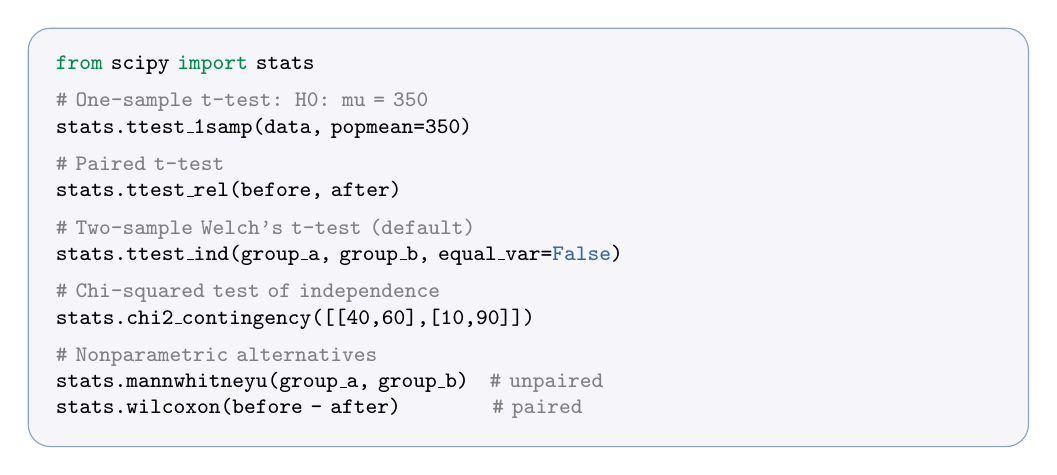
\begin{tikzpicture}
  \node[draw=popblue!60, fill=lightbg, rounded corners=8pt, text width=12cm, align=left, inner sep=10pt, font=\ttfamily\footnotesize] {
    \textcolor{paramgreen}{from} scipy \textcolor{paramgreen}{import} stats\\[4pt]
    \textcolor{gray}{\# One-sample t-test: H0: mu = 350}\\
    stats.ttest\_1samp(data, popmean=350)\\[4pt]
    \textcolor{gray}{\# Paired t-test}\\
    stats.ttest\_rel(before, after)\\[4pt]
    \textcolor{gray}{\# Two-sample Welch's t-test (default)}\\
    stats.ttest\_ind(group\_a, group\_b, equal\_var=\textcolor{popblue}{False})\\[4pt]
    \textcolor{gray}{\# Chi-squared test of independence}\\
    stats.chi2\_contingency([[40,60],[10,90]])\\[4pt]
    \textcolor{gray}{\# Nonparametric alternatives}\\
    stats.mannwhitneyu(group\_a, group\_b) \;\;\textcolor{gray}{\# unpaired}\\
    stats.wilcoxon(before - after) \qquad\quad\;\;\textcolor{gray}{\# paired}
  };
\end{tikzpicture}
\end{center}

\vspace{0.1cm}
\centering\small
Each function returns \texttt{(statistic, p\_value)}. Always check which alternative hypothesis is default.
\end{frame}

% ============================================================
% PART V: THE UNIFYING PICTURE — LRT REVEAL
% ============================================================
\section{The Unifying Picture}

\begin{frame}
\begin{center}
  \vspace{1.2cm}
  {\Huge\bfseries\textcolor{violet1}{Part V: The Unifying Picture}}

  \vspace{0.8cm}
  {\large Wait --- those tests were all the same test in disguise.}

  \vspace{0.4cm}
  {\large The Likelihood Ratio framework}
\end{center}
\end{frame}

% --- NEW: notice the pattern ---
\begin{frame}
\frametitle{Notice the Pattern}

\small
Look back at every test we just saw. They share the same shape:

\vspace{0.15cm}
\begin{center}
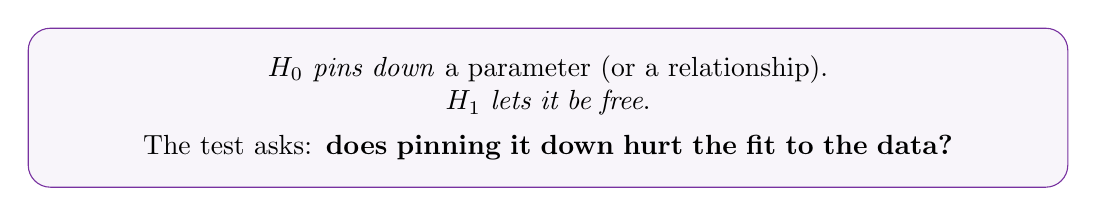
\begin{tikzpicture}
  \node[draw=violet1, fill=violet1!5, rounded corners=8pt, text width=12.5cm, align=center, inner sep=10pt] {
    $H_0$ \emph{pins down} a parameter (or a relationship).\\
    $H_1$ \emph{lets it be free}.\\[4pt]
    The test asks: \textbf{does pinning it down hurt the fit to the data?}
  };
\end{tikzpicture}
\end{center}

\vspace{0.2cm}
\begin{center}
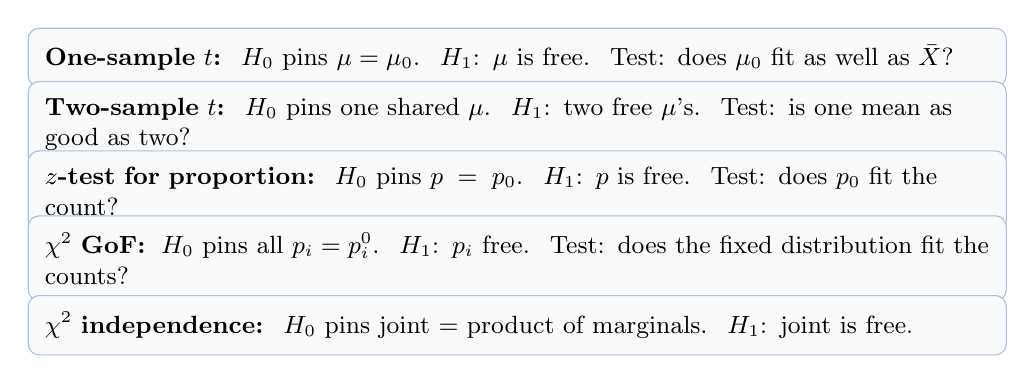
\begin{tikzpicture}[
  rbox/.style={draw=popblue!40, fill=popblue!3, rounded corners=4pt, text width=12cm, align=left, inner sep=6pt, font=\small}
]
  \node[rbox] at (0, 1.7) {\textbf{One-sample $t$:}\; $H_0$ pins $\mu = \mu_0$. \;$H_1$: $\mu$ is free. \;Test: does $\mu_0$ fit as well as $\bar X$?};
  \node[rbox] at (0, 0.85) {\textbf{Two-sample $t$:}\; $H_0$ pins one shared $\mu$. \;$H_1$: two free $\mu$'s. \;Test: is one mean as good as two?};
  \node[rbox] at (0, 0.0) {\textbf{$z$-test for proportion:}\; $H_0$ pins $p = p_0$. \;$H_1$: $p$ is free. \;Test: does $p_0$ fit the count?};
  \node[rbox] at (0, -0.85) {\textbf{$\chi^2$ GoF:}\; $H_0$ pins all $p_i = p_i^0$. \;$H_1$: $p_i$ free. \;Test: does the fixed distribution fit the counts?};
  \node[rbox] at (0, -1.7) {\textbf{$\chi^2$ independence:}\; $H_0$ pins joint $=$ product of marginals. \;$H_1$: joint is free.};
\end{tikzpicture}
\end{center}
\end{frame}

% --- restricted vs full models, NOW anchored on tests they've seen ---
\begin{frame}
\frametitle{Restricted vs Full Models}
\framesubtitle{Putting names on the pattern}

\small
The pattern has names. The ``pinned'' model is \textbf{restricted}; the ``free'' model is \textbf{full}.

\vspace{0.1cm}
\begin{center}
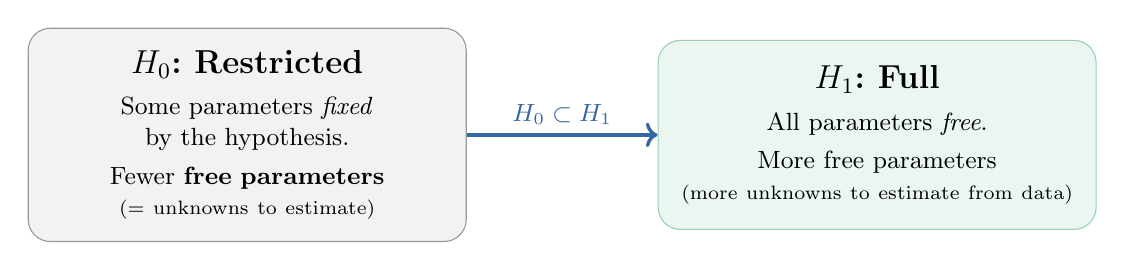
\begin{tikzpicture}[
  mbox/.style={draw, rounded corners=8pt, text width=5cm, align=center, inner sep=8pt, font=\small, minimum height=2.4cm}
]
  \node[mbox, fill=black!5, draw=black!40] (m0) at (-4, 0) {
    {\large\textbf{$H_0$: Restricted}}\\[4pt]
    Some parameters \textit{fixed}\\
    by the hypothesis.\\[3pt]
    Fewer \textbf{free parameters}\\
    {\scriptsize (= unknowns to estimate)}
  };
  \node[mbox, fill=paramgreen!8, draw=paramgreen!40] (m1) at (4, 0) {
    {\large\textbf{$H_1$: Full}}\\[4pt]
    All parameters \textit{free}.\\[3pt]
    More free parameters\\
    {\scriptsize (more unknowns to estimate from data)}
  };
  \draw[->, very thick, popblue] (m0) -- (m1) node[midway, above, font=\small\bfseries] {$H_0 \subset H_1$};
\end{tikzpicture}
\end{center}

\vspace{0.15cm}
\begin{center}
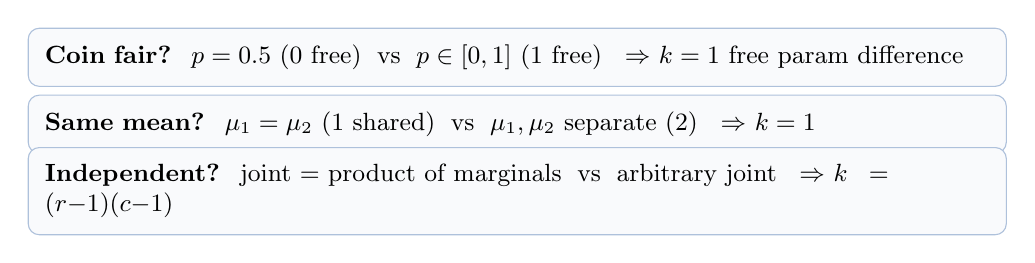
\begin{tikzpicture}[
  ebox/.style={draw=popblue!40, fill=popblue!3, rounded corners=4pt, text width=12cm, align=left, inner sep=6pt, font=\small}
]
  \node[ebox] at (0, 0.85) {\textbf{Coin fair?}\; $p = 0.5$ (0 free) \;vs\; $p \in [0,1]$ (1 free) \;\;$\Rightarrow$ $k = 1$ free param difference};
  \node[ebox] at (0, 0.0) {\textbf{Same mean?}\; $\mu_1 = \mu_2$ (1 shared) \;vs\; $\mu_1, \mu_2$ separate (2) \;\;$\Rightarrow$ $k = 1$};
  \node[ebox] at (0, -0.85) {\textbf{Independent?}\; joint $=$ product of marginals \;vs\; arbitrary joint \;\;$\Rightarrow$ $k = (r{-}1)(c{-}1)$};
\end{tikzpicture}
\end{center}

\vspace{0.05cm}
{\scriptsize\textcolor{gray}{The number $k$ is the count of constraints $H_0$ imposes. It will determine the test's degrees of freedom.}}
\end{frame}

% --- The LRT statistic Lambda (frame 1: definition + interpretation) ---
\begin{frame}
\frametitle{The Likelihood Ratio Statistic $\Lambda$ (1/2)}
\framesubtitle{Definition and interpretation}

\small
\textbf{Recipe:} fit both models using MLE (Lecture~5), then compare how well they fit.

\vspace{0.05cm}
\begin{center}
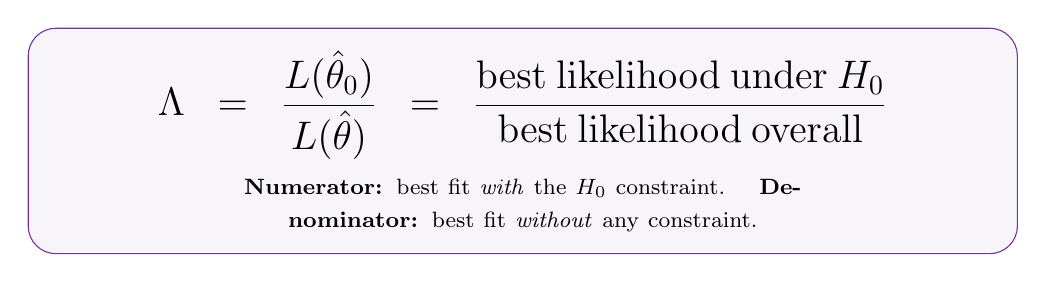
\begin{tikzpicture}
  \node[draw=violet1, fill=violet1!5, rounded corners=10pt, text width=12cm, align=center, inner sep=8pt] {
    {\Large $\Lambda = \dfrac{L(\hat\theta_0)}{L(\hat\theta)} = \dfrac{\text{best likelihood under }H_0}{\text{best likelihood overall}}$}\\[6pt]
    \footnotesize
    \textbf{Numerator:} best fit \emph{with} the $H_0$ constraint. \;
    \textbf{Denominator:} best fit \emph{without} any constraint.
  };
\end{tikzpicture}
\end{center}

\vspace{0.05cm}
\small Denominator $\geq$ numerator (more freedom $\Rightarrow$ better fit), so $0 \leq \Lambda \leq 1$.

\vspace{0.1cm}
\begin{center}
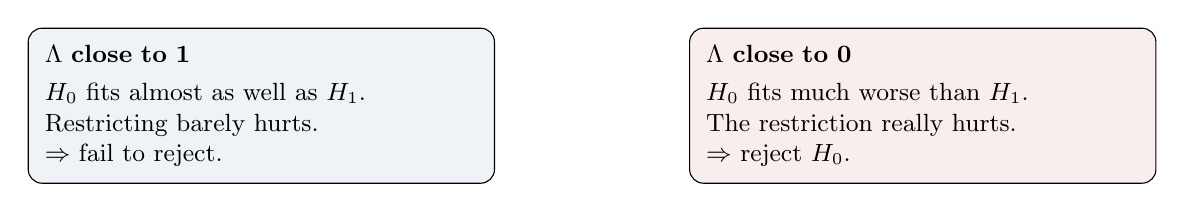
\begin{tikzpicture}[
  ebox/.style={draw, rounded corners=5pt, text width=5.5cm, align=left, inner sep=6pt, font=\small, minimum height=1.8cm}
]
  \node[ebox, fill=popblue!8] at (-4.2, 0) {
    \textbf{$\Lambda$ close to 1}\\[3pt]
    $H_0$ fits almost as well as $H_1$.\\
    Restricting barely hurts.\\
    $\Rightarrow$ fail to reject.
  };
  \node[ebox, fill=warnred!8] at (4.2, 0) {
    \textbf{$\Lambda$ close to 0}\\[3pt]
    $H_0$ fits much worse than $H_1$.\\
    The restriction really hurts.\\
    $\Rightarrow$ reject $H_0$.
  };
\end{tikzpicture}
\end{center}
\end{frame}

% --- The LRT statistic Lambda (frame 2: why -2 log Lambda) ---
\begin{frame}
\frametitle{The Likelihood Ratio Statistic $\Lambda$ (2/2)}
\framesubtitle{Why we transform to $-2\log\Lambda$}

\small
$\Lambda$ is awkward to work with directly. We use $-2\log\Lambda$ instead. Three reasons:

\vspace{0.2cm}
\begin{center}
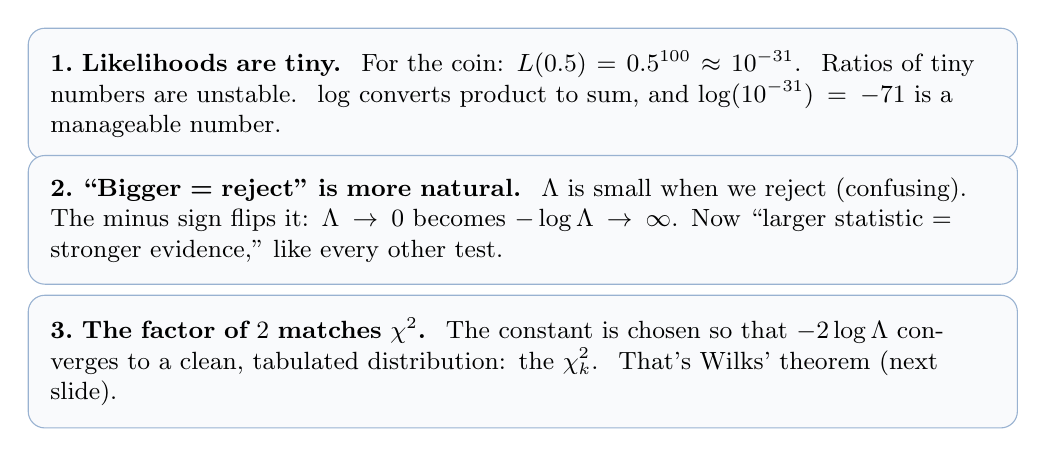
\begin{tikzpicture}[
  rbox/.style={draw=popblue!50, fill=popblue!3, rounded corners=6pt, text width=12cm, align=left, inner sep=8pt, font=\small}
]
  \node[rbox] at (0, 2.0) {
    \textbf{1.\ Likelihoods are tiny.}\;
    For the coin: $L(0.5) = 0.5^{100} \approx 10^{-31}$. \;Ratios of tiny numbers are unstable. \;$\log$ converts product to sum, and $\log(10^{-31}) = -71$ is a manageable number.
  };
  \node[rbox] at (0, 0.4) {
    \textbf{2.\ ``Bigger = reject'' is more natural.}\;
    $\Lambda$ is small when we reject (confusing). The minus sign flips it: $\Lambda \to 0$ becomes $-\log\Lambda \to \infty$. Now ``larger statistic = stronger evidence,'' like every other test.
  };
  \node[rbox] at (0, -1.4) {
    \textbf{3.\ The factor of $2$ matches $\chi^2$.}\;
    The constant is chosen so that $-2\log\Lambda$ converges to a clean, tabulated distribution: the $\chi^2_k$. \;That's Wilks' theorem (next slide).
  };
\end{tikzpicture}
\end{center}

\vspace{0.15cm}
\begin{center}
\fcolorbox{violet1}{violet1!5}{\parbox{10cm}{\centering\small
  Bottom line: $-2\log\Lambda \geq 0$. \;Reject when it's large.
}}
\end{center}
\end{frame}

% --- worked LRT: coin (REVIVED, full computation) ---
\begin{frame}
\frametitle{Worked LRT: The Coin, End to End}

\small
\textbf{Data:} 100 flips, 62 heads. \;$H_0\!: p = 0.5$ vs $H_1\!: p \in [0,1]$ \;($k = 1$ free-param diff).

\vspace{0.15cm}
\begin{center}
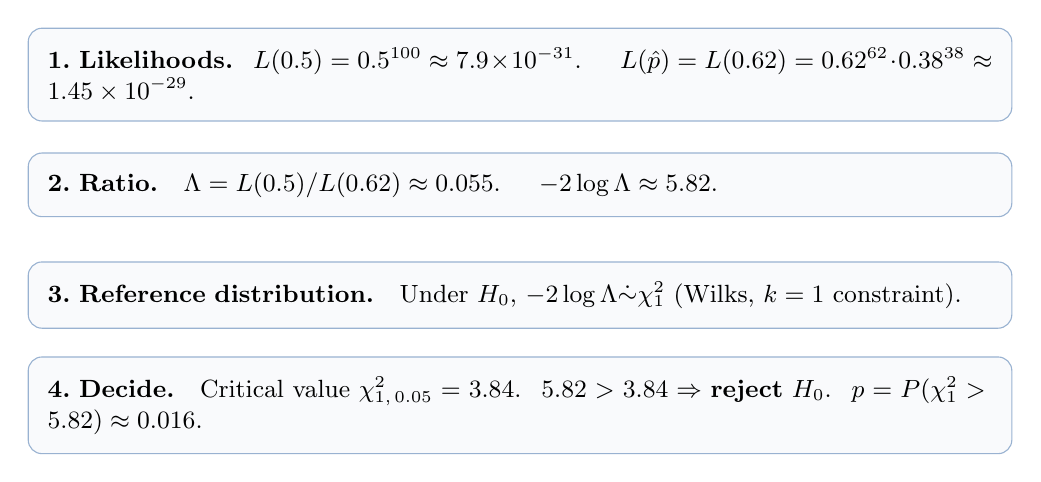
\begin{tikzpicture}[
  lrtstep/.style={draw=popblue!50, fill=popblue!3, rounded corners=5pt, text width=12cm, align=left, inner sep=7pt, font=\small}
]
  \node[lrtstep] at (0, 2.4) {
    \textbf{1.\ Likelihoods.}\;
    $L(0.5) = 0.5^{100} \approx 7.9 \times 10^{-31}$. \quad
    $L(\hat p) = L(0.62) = 0.62^{62} \cdot 0.38^{38} \approx 1.45 \times 10^{-29}$.
  };
  \node[lrtstep] at (0, 1.0) {
    \textbf{2.\ Ratio.}\quad
    $\Lambda = L(0.5)/L(0.62) \approx 0.055$. \quad
    $-2\log\Lambda \approx 5.82$.
  };
  \node[lrtstep] at (0, -0.4) {
    \textbf{3.\ Reference distribution.}\quad
    Under $H_0$, $-2\log\Lambda \dot\sim \chi^2_1$ (Wilks, $k = 1$ constraint).
  };
  \node[lrtstep] at (0, -1.8) {
    \textbf{4.\ Decide.}\quad
    Critical value $\chi^2_{1,\,0.05} = 3.84$. \;$5.82 > 3.84 \Rightarrow$ \textbf{reject} $H_0$. \;$p = P(\chi^2_1 > 5.82) \approx 0.016$.
  };
\end{tikzpicture}
\end{center}

\vspace{0.15cm}
\begin{center}
\fcolorbox{paramgreen}{paramgreen!5}{\parbox{12cm}{\centering\footnotesize
  \textbf{Sanity check (same data):} $z$-test gives $Z = 2.40$, $Z^2 = 5.76$, $p \approx 0.016$. Same answer --- the $z$-test \textbf{is} this LRT in disguise.
}}
\end{center}
\end{frame}

% --- Wilks' theorem (now with backward references to seen tests) ---
\begin{frame}
\frametitle{Wilks' Theorem: Why It All Works}

\small
The reason every test today produced a valid $p$-value is one theorem. Under $H_0$, as $n \to \infty$:

\vspace{0.1cm}
\begin{center}
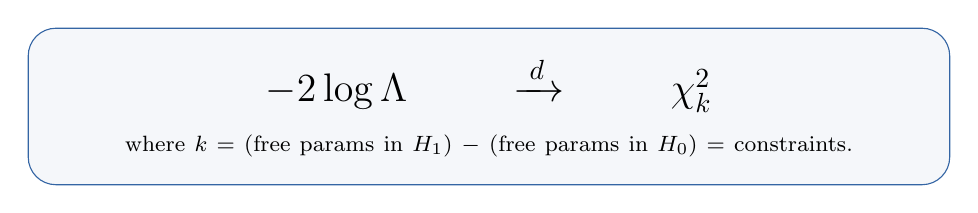
\begin{tikzpicture}
  \node[draw=popblue, fill=popblue!5, rounded corners=10pt, text width=11cm, align=center, inner sep=10pt] {
    {\Large $-2\log\Lambda \;\xrightarrow{\;d\;}\; \chi^2_k$}\\[6pt]
    \footnotesize where $k$ = (free params in $H_1$) $-$ (free params in $H_0$) = constraints.
  };
\end{tikzpicture}
\end{center}

\vspace{0.1cm}
The tests we already saw, retroactively explained:

\vspace{0.05cm}
\begin{center}
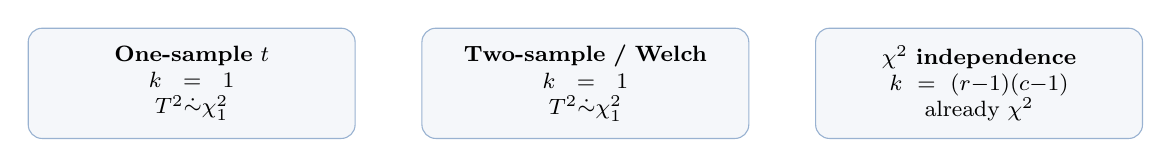
\begin{tikzpicture}[
  kbox/.style={draw=popblue!50, fill=popblue!5, rounded corners=5pt, text width=3.8cm, align=center, inner sep=5pt, font=\footnotesize, minimum height=1.4cm}
]
  \node[kbox] at (-5, 0) {\textbf{One-sample $t$}\\$k = 1$\\$T^2 \dot\sim \chi^2_1$};
  \node[kbox] at (0, 0) {\textbf{Two-sample / Welch}\\$k = 1$\\$T^2 \dot\sim \chi^2_1$};
  \node[kbox] at (5, 0) {\textbf{$\chi^2$ independence}\\$k = (r{-}1)(c{-}1)$\\already $\chi^2$};
\end{tikzpicture}
\end{center}

\vspace{0.1cm}
\begin{center}
\fcolorbox{orange1}{orange1!5}{\parbox{11.5cm}{\centering\footnotesize
  \textbf{The takeaway:} every test today is an LRT on nested models, and Wilks tells you what distribution to compare against. \;\textbf{Caveat:} asymptotic. For small $n$, prefer exact tests (Fisher, binomial).
}}
\end{center}
\end{frame}

% ============================================================
\section{Mid-deck Recap}

\begin{frame}
\frametitle{Recap: Classical Tests \& LRT}
\begin{center}
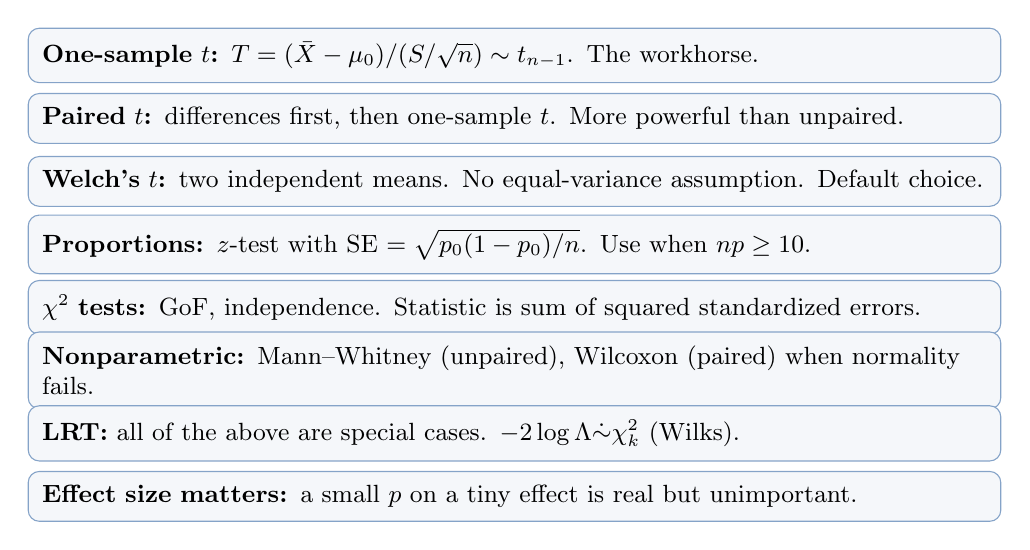
\begin{tikzpicture}[
  sbox/.style={draw=popblue!60, fill=popblue!5, rounded corners=4pt, text width=12cm, minimum height=0.5cm, align=left, inner sep=5pt, font=\small}
]
  \node[sbox] at (0, 3.2) {\textbf{One-sample $t$:} $T = (\bar{X} - \mu_0)/(S/\sqrt{n}) \sim t_{n-1}$. The workhorse.};
  \node[sbox] at (0, 2.4) {\textbf{Paired $t$:} differences first, then one-sample $t$. More powerful than unpaired.};
  \node[sbox] at (0, 1.6) {\textbf{Welch's $t$:} two independent means. No equal-variance assumption. Default choice.};
  \node[sbox] at (0, 0.8) {\textbf{Proportions:} $z$-test with SE $= \sqrt{p_0(1-p_0)/n}$. Use when $np \geq 10$.};
  \node[sbox] at (0, 0.0) {\textbf{$\chi^2$ tests:} GoF, independence. Statistic is sum of squared standardized errors.};
  \node[sbox] at (0, -0.8) {\textbf{Nonparametric:} Mann--Whitney (unpaired), Wilcoxon (paired) when normality fails.};
  \node[sbox] at (0, -1.6) {\textbf{LRT:} all of the above are special cases. $-2\log\Lambda \dot\sim \chi^2_k$ (Wilks).};
  \node[sbox] at (0, -2.4) {\textbf{Effect size matters:} a small $p$ on a tiny effect is real but unimportant.};
\end{tikzpicture}
\end{center}

\vspace{0.2cm}
\begin{center}
{\large\textbf{Up next:}} What if we have \textbf{three or more} groups? And how does industry actually run experiments?
\end{center}
\end{frame}

% ============================================================
% PART VI: FROM 2 TO k GROUPS — ANOVA
% ============================================================
\section{From 2 to k Groups: ANOVA}

\begin{frame}
\begin{center}
  \vspace{1.5cm}
  {\Huge\bfseries\textcolor{popblue}{Part VI: From 2 to $k$ Groups}}

  \vspace{0.8cm}
  {\large Three groups, three $t$-tests --- what could go wrong?}
\end{center}
\end{frame}

\begin{frame}
\frametitle{Comparing More Than Two Groups}

\small
\textbf{Scenario:} A teacher tries three teaching methods (A, B, C) on different classes. Are exam scores different?

\vspace{0.2cm}
\begin{center}
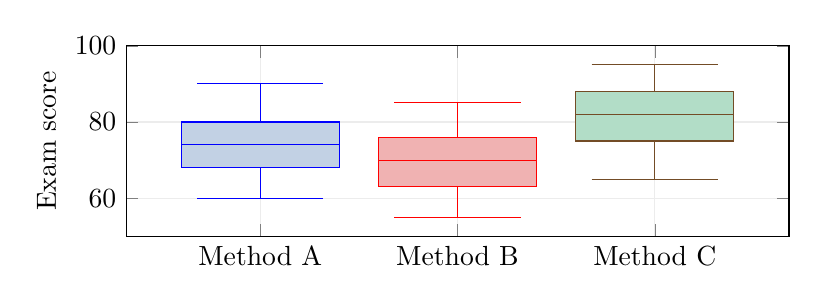
\begin{tikzpicture}
  \begin{axis}[
    width=10cm, height=4cm,
    boxplot/draw direction=y,
    xtick={1, 2, 3},
    xticklabels={Method A, Method B, Method C},
    ylabel={Exam score},
    ymin=50, ymax=100,
    grid=major, grid style={gray!15},
    every axis plot/.style={fill=popblue!25}
  ]
    \addplot+[boxplot prepared={lower whisker=60, lower quartile=68, median=74, upper quartile=80, upper whisker=90}, fill=popblue!30] coordinates {};
    \addplot+[boxplot prepared={lower whisker=55, lower quartile=63, median=70, upper quartile=76, upper whisker=85}, fill=sampred!30] coordinates {};
    \addplot+[boxplot prepared={lower whisker=65, lower quartile=75, median=82, upper quartile=88, upper whisker=95}, fill=paramgreen!30] coordinates {};
  \end{axis}
\end{tikzpicture}
\end{center}

\vspace{0.1cm}
\textbf{Na\"ive approach:} Run three pairwise $t$-tests: A vs B, A vs C, B vs C.

\vspace{0.1cm}
\textbf{Problem:} Each test has $\alpha = 0.05$ false positive rate. Three tests?
$$P(\text{at least one false positive}) = 1 - (1 - 0.05)^3 = 0.143$$
With 10 groups: $\binom{10}{2} = 45$ tests $\Rightarrow$ $1 - 0.95^{45} = 0.90$. Almost certain to find ``something.''
\end{frame}

\begin{frame}
\frametitle{The Multiple Comparisons Explosion}

\begin{center}
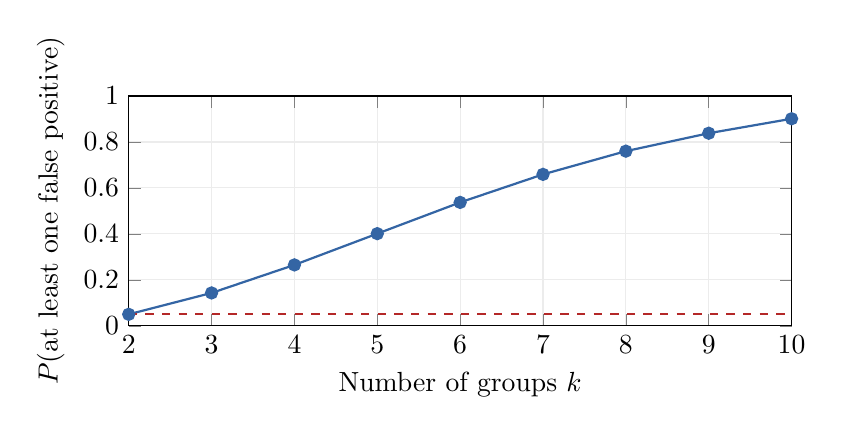
\begin{tikzpicture}
  \begin{axis}[
    width=10cm, height=4.5cm,
    xlabel={Number of groups $k$},
    ylabel={$P(\text{at least one false positive})$},
    xmin=2, xmax=10,
    ymin=0, ymax=1,
    grid=major, grid style={gray!15},
    xtick={2,3,4,5,6,7,8,9,10},
    ytick={0, 0.2, 0.4, 0.6, 0.8, 1.0},
    every axis plot/.style={thick, mark=*, mark size=2pt}
  ]
    \addplot[popblue] coordinates {
      (2, 0.05) (3, 0.143) (4, 0.265) (5, 0.401) (6, 0.537)
      (7, 0.659) (8, 0.760) (9, 0.838) (10, 0.901)
    };
    \draw[thick, dashed, warnred] (axis cs:2, 0.05) -- (axis cs:10, 0.05);
    \node[font=\scriptsize, warnred, right] at (axis cs:10, 0.08) {$\alpha = 0.05$};
  \end{axis}
\end{tikzpicture}
\end{center}

\vspace{0.1cm}
\begin{center}
\fcolorbox{warnred}{warnred!5}{\parbox{10cm}{\centering\small
  \textbf{We need a single test} that asks: ``Are \emph{any} of these group means different?''\\
  while controlling the overall Type~I error rate at $\alpha$.\\[3pt]
  That test is \textbf{ANOVA} (Analysis of Variance).
}}
\end{center}
\end{frame}

\begin{frame}
\frametitle{The Core Idea: Between vs Within}

\begin{center}
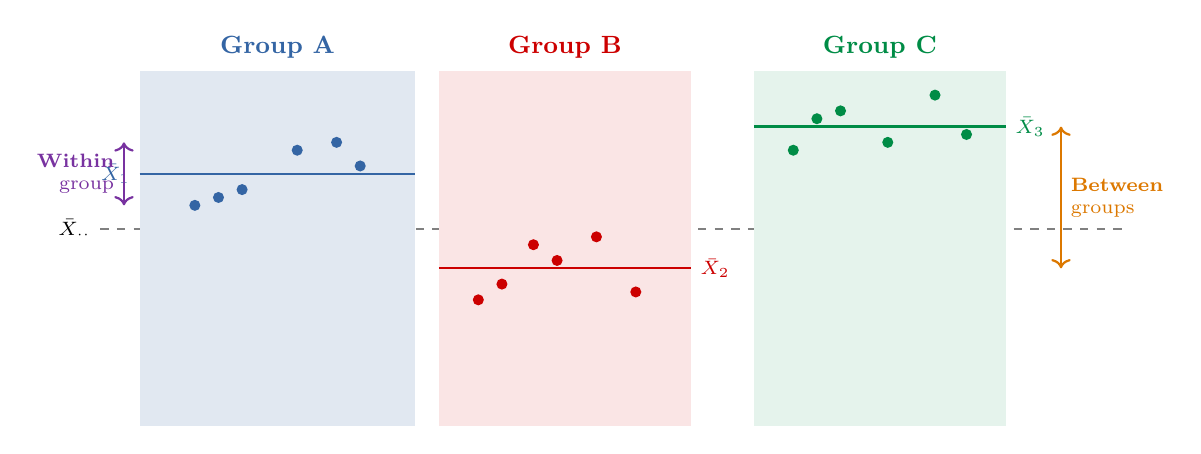
\begin{tikzpicture}
  \draw[thick, dashed, black!50] (0, 2.5) -- (13, 2.5);
  \node[font=\scriptsize, left] at (0, 2.5) {$\bar{X}_{\cdot\cdot}$};

  \fill[popblue!15] (0.5, 0) rectangle (4, 4.5);
  \node[font=\small\bfseries, popblue] at (2.25, 4.8) {Group A};
  \draw[thick, popblue] (0.5, 3.2) -- (4, 3.2);
  \node[font=\scriptsize, popblue, left] at (0.5, 3.2) {$\bar{X}_1$};
  \foreach \x/\y in {1.2/2.8, 1.8/3.0, 2.5/3.5, 3.0/3.6, 1.5/2.9, 3.3/3.3} {
    \fill[popblue] (\x, \y) circle (2pt);
  }

  \fill[sampred!10] (4.3, 0) rectangle (7.5, 4.5);
  \node[font=\small\bfseries, sampred] at (5.9, 4.8) {Group B};
  \draw[thick, sampred] (4.3, 2.0) -- (7.5, 2.0);
  \node[font=\scriptsize, sampred, right] at (7.5, 2.0) {$\bar{X}_2$};
  \foreach \x/\y in {4.8/1.6, 5.5/2.3, 5.1/1.8, 6.3/2.4, 5.8/2.1, 6.8/1.7} {
    \fill[sampred] (\x, \y) circle (2pt);
  }

  \fill[paramgreen!10] (8.3, 0) rectangle (11.5, 4.5);
  \node[font=\small\bfseries, paramgreen] at (9.9, 4.8) {Group C};
  \draw[thick, paramgreen] (8.3, 3.8) -- (11.5, 3.8);
  \node[font=\scriptsize, paramgreen, right] at (11.5, 3.8) {$\bar{X}_3$};
  \foreach \x/\y in {8.8/3.5, 9.4/4.0, 10.0/3.6, 10.6/4.2, 9.1/3.9, 11.0/3.7} {
    \fill[paramgreen] (\x, \y) circle (2pt);
  }

  \draw[<->, thick, orange1] (12.2, 2.0) -- (12.2, 3.8);
  \node[font=\scriptsize, orange1, right, align=left] at (12.2, 2.9) {\textbf{Between}\\groups};

  \draw[<->, thick, violet1] (0.3, 2.8) -- (0.3, 3.6);
  \node[font=\scriptsize, violet1, left, align=right] at (0.3, 3.2) {\textbf{Within}\\group};
\end{tikzpicture}
\end{center}

\vspace{0.1cm}
\begin{center}
\fcolorbox{popblue}{popblue!5}{\parbox{11cm}{\centering\small
  \textbf{If group means are truly equal,} the ``between-group'' variability should be\\
  no larger than the ``within-group'' variability (just random noise).
}}
\end{center}
\end{frame}

\begin{frame}
\frametitle{Sum of Squares Decomposition}

\vspace{-0.1cm}
\begin{center}
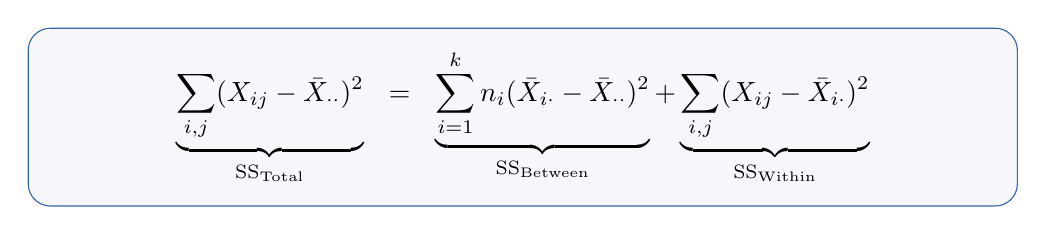
\begin{tikzpicture}
  \node[draw=popblue, fill=popblue!5, rounded corners=8pt, text width=12cm, align=center, inner sep=8pt] {
    $\underbrace{\sum_{i,j}(X_{ij} - \bar{X}_{\cdot\cdot})^2}_{\text{SS}_{\text{Total}}} = \underbrace{\sum_{i=1}^{k} n_i(\bar{X}_{i\cdot} - \bar{X}_{\cdot\cdot})^2}_{\text{SS}_{\text{Between}}} + \underbrace{\sum_{i,j}(X_{ij} - \bar{X}_{i\cdot})^2}_{\text{SS}_{\text{Within}}}$
  };
\end{tikzpicture}
\end{center}

\vspace{0.1cm}
\begin{center}
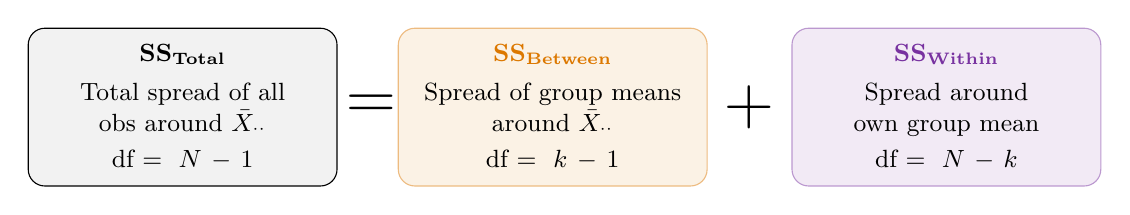
\begin{tikzpicture}[
  cbox/.style={draw, rounded corners=6pt, text width=3.5cm, align=center, inner sep=6pt, font=\small, minimum height=1.8cm}
]
  \node[cbox, fill=black!5] at (-5.2, 0) {
    {\bfseries $\text{SS}_{\text{Total}}$}\\[3pt]
    Total spread of all\\
    obs around $\bar{X}_{\cdot\cdot}$\\[2pt]
    df $= N - 1$
  };
  \node[font=\Huge] at (-2.8, 0) {$=$};
  \node[cbox, fill=orange1!10, draw=orange1!50] at (-0.5, 0) {
    {\bfseries\textcolor{orange1}{$\text{SS}_{\text{Between}}$}}\\[3pt]
    Spread of group means\\
    around $\bar{X}_{\cdot\cdot}$\\[2pt]
    df $= k - 1$
  };
  \node[font=\Huge] at (2, 0) {$+$};
  \node[cbox, fill=violet1!10, draw=violet1!50] at (4.5, 0) {
    {\bfseries\textcolor{violet1}{$\text{SS}_{\text{Within}}$}}\\[3pt]
    Spread around\\
    own group mean\\[2pt]
    df $= N - k$
  };
\end{tikzpicture}
\end{center}

\vspace{0.15cm}
\begin{center}
\fcolorbox{popblue}{popblue!5}{\parbox{11cm}{\centering\small
  \textbf{Concrete example (3 methods, $N=30$, used on the next slide):}\\[2pt]
  $\text{SS}_\text{Total} = 1800$, \quad $\text{SS}_\text{Between} = 720$ (df $= 2$), \quad $\text{SS}_\text{Within} = 1080$ (df $= 27$).
}}
\end{center}
\end{frame}

\begin{frame}
\frametitle{The $F$-Statistic}

\begin{center}
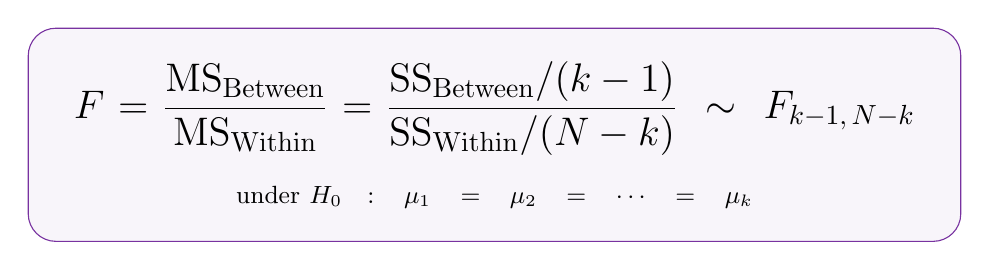
\begin{tikzpicture}
  \node[draw=violet1, fill=violet1!5, rounded corners=10pt, text width=11cm, align=center, inner sep=12pt] {
    {\Large $F = \dfrac{\text{MS}_{\text{Between}}}{\text{MS}_{\text{Within}}} = \dfrac{\text{SS}_{\text{Between}} / (k - 1)}{\text{SS}_{\text{Within}} / (N - k)} \;\sim\; F_{k-1,\, N-k}$}\\[10pt]
    \small under $H_0\!: \mu_1 = \mu_2 = \cdots = \mu_k$
  };
\end{tikzpicture}
\end{center}

\vspace{0.2cm}
\begin{center}
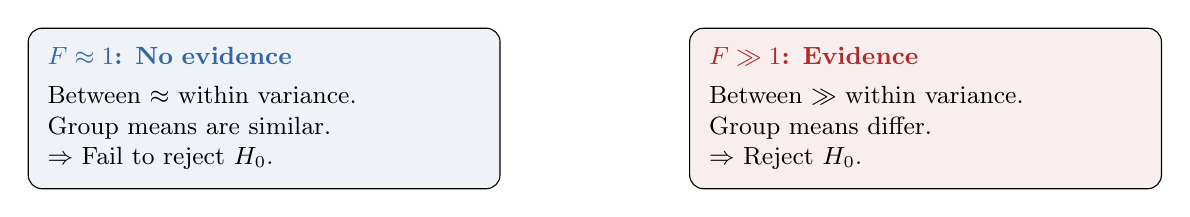
\begin{tikzpicture}[
  cbox/.style={draw, rounded corners=5pt, text width=5.5cm, align=left, inner sep=7pt, font=\small}
]
  \node[cbox, fill=popblue!8] at (-4.2, 0) {
    \textbf{\textcolor{popblue}{$F \approx 1$: No evidence}}\\[3pt]
    Between $\approx$ within variance.\\
    Group means are similar.\\
    $\Rightarrow$ Fail to reject $H_0$.
  };
  \node[cbox, fill=warnred!8] at (4.2, 0) {
    \textbf{\textcolor{warnred}{$F \gg 1$: Evidence}}\\[3pt]
    Between $\gg$ within variance.\\
    Group means differ.\\
    $\Rightarrow$ Reject $H_0$.
  };
\end{tikzpicture}
\end{center}

\vspace{0.1cm}
\begin{center}
\small $F$ is always $\geq 0$. We only reject in the \textbf{right tail} (one-sided).
\end{center}
\end{frame}

\begin{frame}
\frametitle{The $F$-Distribution}

\begin{center}
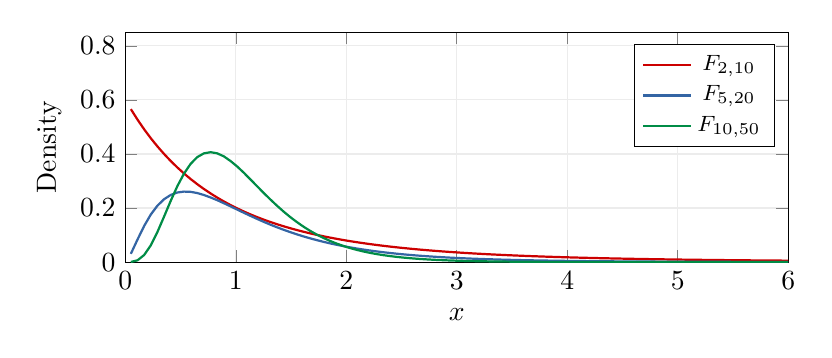
\begin{tikzpicture}
  \begin{axis}[
    width=10cm, height=4.5cm,
    domain=0.05:6, samples=100,
    xlabel={$x$}, ylabel={Density},
    xmin=0, xmax=6, ymin=0, ymax=0.85,
    grid=major, grid style={gray!15},
    legend style={at={(0.98,0.95)}, anchor=north east, font=\footnotesize},
    every axis plot/.style={thick, no markers}
  ]
    \addplot[sampred] {(1/(1+x*2/10))^6 * (x*2/10)^0 * 2/10 / 0.333};
    \addlegendentry{$F_{2,10}$}
    \addplot[popblue] {x^(1.5) * (1+x*5/20)^(-12.5) * 3.2};
    \addlegendentry{$F_{5,20}$}
    \addplot[paramgreen] {x^(4) * (1+x*10/50)^(-30) * 85};
    \addlegendentry{$F_{10,50}$}
  \end{axis}
\end{tikzpicture}
\end{center}

\vspace{0.1cm}
\begin{center}
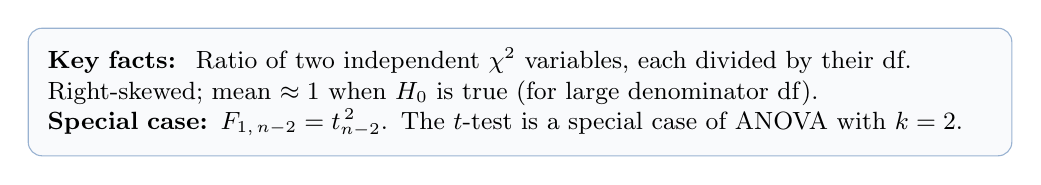
\begin{tikzpicture}
  \node[draw=popblue!50, fill=popblue!3, rounded corners=5pt, text width=12cm, align=left, inner sep=7pt, font=\small] {
    \textbf{Key facts:}\;
    Ratio of two independent $\chi^2$ variables, each divided by their df.\\
    Right-skewed; mean $\approx 1$ when $H_0$ is true (for large denominator df).\\
    \textbf{Special case:} $F_{1,\,n-2} = t_{n-2}^{\,2}$. The $t$-test is a special case of ANOVA with $k = 2$.
  };
\end{tikzpicture}
\end{center}
\end{frame}

\begin{frame}
\frametitle{The ANOVA Table}

\begin{center}
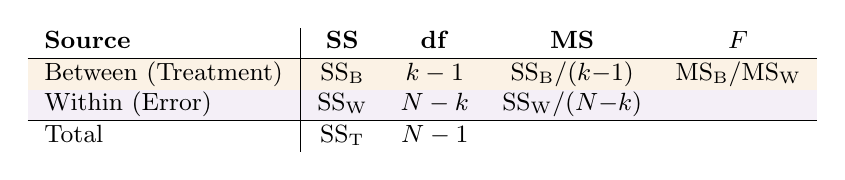
\begin{tikzpicture}
  \node[inner sep=0pt] {
    \small
    \begin{tabular}{l|cccc}
      \textbf{Source} & \textbf{SS} & \textbf{df} & \textbf{MS} & \textbf{$F$} \\
      \hline
      \rowcolor{orange1!10}
      Between (Treatment) & $\text{SS}_\text{B}$ & $k - 1$ & $\text{SS}_\text{B}/(k{-}1)$ & $\text{MS}_\text{B}/\text{MS}_\text{W}$ \\
      \rowcolor{violet1!8}
      Within (Error) & $\text{SS}_\text{W}$ & $N - k$ & $\text{SS}_\text{W}/(N{-}k)$ & \\
      \hline
      Total & $\text{SS}_\text{T}$ & $N - 1$ & & \\
    \end{tabular}
  };
\end{tikzpicture}
\end{center}

\vspace{0.3cm}
\textbf{Example:} the three teaching methods, $n_i = 10$ each ($N = 30$), with the $\text{SS}$ values from two slides ago.

\vspace{0.1cm}
\begin{center}
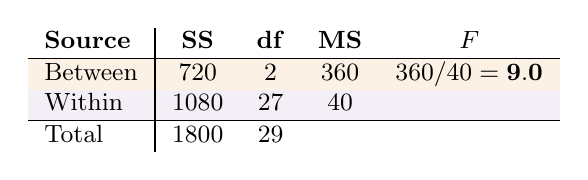
\begin{tikzpicture}
  \node[inner sep=0pt] {
    \small
    \begin{tabular}{l|cccc}
      \textbf{Source} & \textbf{SS} & \textbf{df} & \textbf{MS} & \textbf{$F$} \\
      \hline
      \rowcolor{orange1!10}
      Between & 720 & 2 & 360 & $360/40 = \mathbf{9.0}$ \\
      \rowcolor{violet1!8}
      Within & 1080 & 27 & 40 & \\
      \hline
      Total & 1800 & 29 & & \\
    \end{tabular}
  };
\end{tikzpicture}
\end{center}

\vspace{0.15cm}
$F_{2,\,27,\,0.05} = 3.35$. Since $F = 9.0 > 3.35$: \textbf{reject} $H_0$.\\
At least one teaching method gives different results. But which one?
\end{frame}

\begin{frame}
\frametitle{ANOVA: Assumptions}

\begin{center}
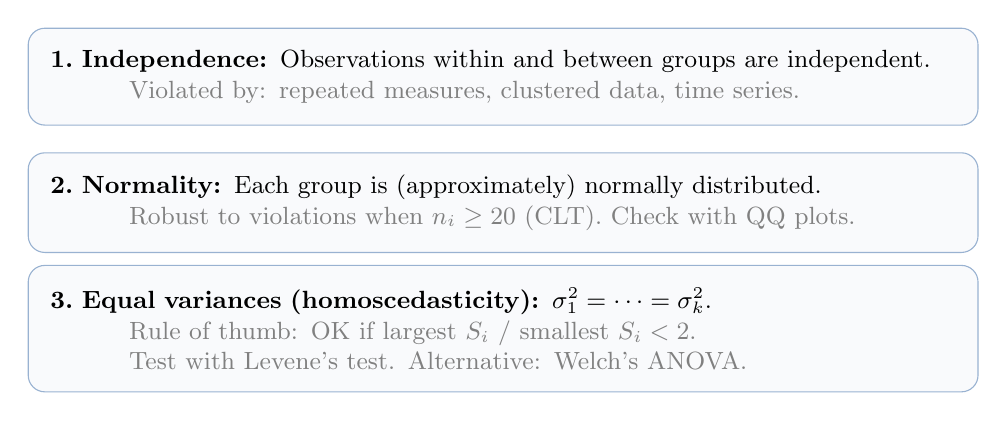
\begin{tikzpicture}[
  abox/.style={draw=popblue!50, fill=popblue!3, rounded corners=6pt, text width=11.5cm, align=left, inner sep=8pt, font=\small}
]
  \node[abox] at (0, 2.6) {
    \textbf{1.\ Independence:} Observations within and between groups are independent.\\
    \hspace{1cm}\textcolor{black!50}{\small Violated by: repeated measures, clustered data, time series.}
  };
  \node[abox] at (0, 1.0) {
    \textbf{2.\ Normality:} Each group is (approximately) normally distributed.\\
    \hspace{1cm}\textcolor{black!50}{\small Robust to violations when $n_i \geq 20$ (CLT). Check with QQ plots.}
  };
  \node[abox] at (0, -0.6) {
    \textbf{3.\ Equal variances (homoscedasticity):} $\sigma_1^2 = \cdots = \sigma_k^2$.\\
    \hspace{1cm}\textcolor{black!50}{\small Rule of thumb: OK if largest $S_i$ / smallest $S_i < 2$.}\\
    \hspace{1cm}\textcolor{black!50}{\small Test with Levene's test. Alternative: Welch's ANOVA.}
  };
\end{tikzpicture}
\end{center}

\vspace{0.2cm}
\begin{center}
\fcolorbox{orange1}{orange1!5}{\parbox{10cm}{\centering\footnotesize
  \textbf{If equal-variance assumption fails:} use \textbf{Welch's ANOVA} (\texttt{pingouin.welch\_anova}).\\
  Note: \texttt{scipy.stats.f\_oneway} does \emph{standard} ANOVA (assumes equal variances).\\
  \textbf{Post-hoc for unequal variances:} \textbf{Games--Howell} instead of Tukey HSD.\\
  If normality fails: use \textbf{Kruskal--Wallis test} (nonparametric ANOVA).
}}
\end{center}
\end{frame}

\begin{frame}
\frametitle{Post-Hoc: Tukey's HSD vs Bonferroni}
\framesubtitle{Only run post-hoc tests \emph{after} ANOVA rejects $H_0$}

\small
ANOVA told us \emph{some} group means differ. Now we ask: \emph{which pairs?} Two standard methods:

\vspace{0.15cm}
\begin{center}
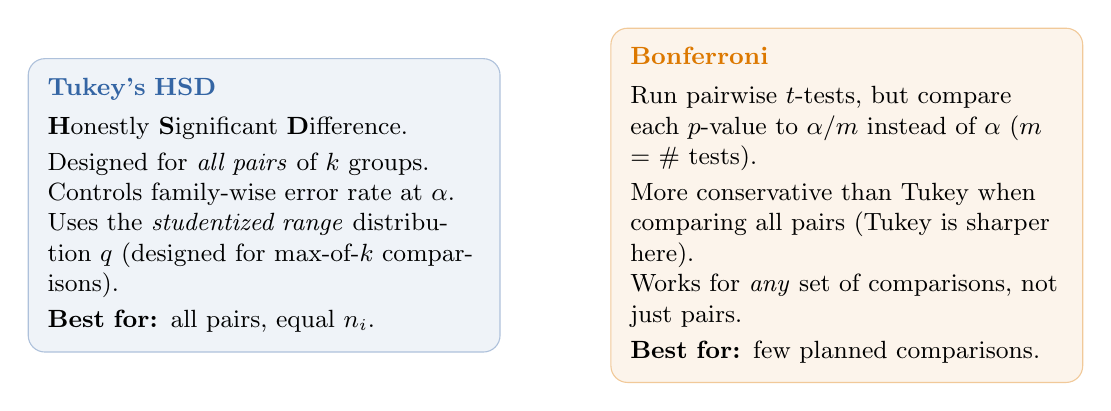
\begin{tikzpicture}[
  cbox/.style={draw, rounded corners=6pt, text width=5.5cm, align=left, inner sep=7pt, font=\small, minimum height=3.6cm}
]
  \node[cbox, fill=popblue!8, draw=popblue!40] at (-3.7, 0) {
    {\bfseries\textcolor{popblue}{Tukey's HSD}}\\[3pt]
    \textbf{H}onestly \textbf{S}ignificant \textbf{D}ifference.\\[2pt]
    Designed for \emph{all pairs} of $k$ groups.\\
    Controls family-wise error rate at $\alpha$.\\
    Uses the \emph{studentized range} distribution $q$ (designed for max-of-$k$ comparisons).\\[2pt]
    \textbf{Best for:} all pairs, equal $n_i$.
  };
  \node[cbox, fill=orange1!8, draw=orange1!40] at (3.7, 0) {
    {\bfseries\textcolor{orange1}{Bonferroni}}\\[3pt]
    Run pairwise $t$-tests, but compare each $p$-value to $\alpha / m$ instead of $\alpha$ ($m$ = \# tests).\\[2pt]
    More conservative than Tukey when comparing all pairs (Tukey is sharper here).\\
    Works for \emph{any} set of comparisons, not just pairs.\\[2pt]
    \textbf{Best for:} few planned comparisons.
  };
\end{tikzpicture}
\end{center}
\end{frame}

\begin{frame}
\frametitle{Tukey's HSD: Worked Example}
\framesubtitle{Three teaching methods (means $74, 70, 82$, $\text{MS}_\text{W} = 40$, $n_i = 10$, df $= 27$)}

\small
\textbf{Step 1.} Compute the HSD threshold. Look up $q_{\alpha,\,k,\,\text{df}}$ for $\alpha = 0.05$, $k = 3$ groups, df $= 27$:
$$q_{0.05,\,3,\,27} \approx 3.51 \quad \text{(studentized range table)}$$

\textbf{Step 2.} Convert to a difference-of-means threshold:
$$\text{HSD} = q \cdot \sqrt{\frac{\text{MS}_\text{W}}{n}} = 3.51 \cdot \sqrt{\frac{40}{10}} = 3.51 \cdot 2 = \mathbf{7.02}$$

\textbf{Step 3.} Any pair of group means whose absolute difference exceeds $7.02$ is significantly different.

\vspace{0.1cm}
\begin{center}
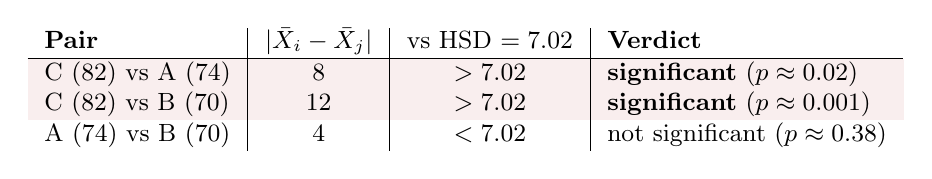
\begin{tikzpicture}
  \node[font=\small, inner sep=0pt] {
    \begin{tabular}{l|c|c|l}
      \textbf{Pair} & $|\bar X_i - \bar X_j|$ & vs HSD $= 7.02$ & \textbf{Verdict} \\
      \hline
      \rowcolor{warnred!8}
      C ($82$) vs A ($74$) & $8$ & $> 7.02$ & \textbf{significant} ($p \approx 0.02$) \\
      \rowcolor{warnred!8}
      C ($82$) vs B ($70$) & $12$ & $> 7.02$ & \textbf{significant} ($p \approx 0.001$) \\
      A ($74$) vs B ($70$) & $4$ & $< 7.02$ & not significant ($p \approx 0.38$) \\
    \end{tabular}
  };
\end{tikzpicture}
\end{center}

\vspace{0.1cm}
\textbf{Conclusion:} Method C beats both A and B. A and B are statistically indistinguishable.

\vspace{0.05cm}
{\scriptsize\textcolor{gray}{In Python: \texttt{from statsmodels.stats.multicomp import pairwise\_tukeyhsd}; \texttt{pairwise\_tukeyhsd(scores, group\_labels)}.}}
\end{frame}

\begin{frame}
\frametitle{Visualizing Post-Hoc Results}

\begin{center}
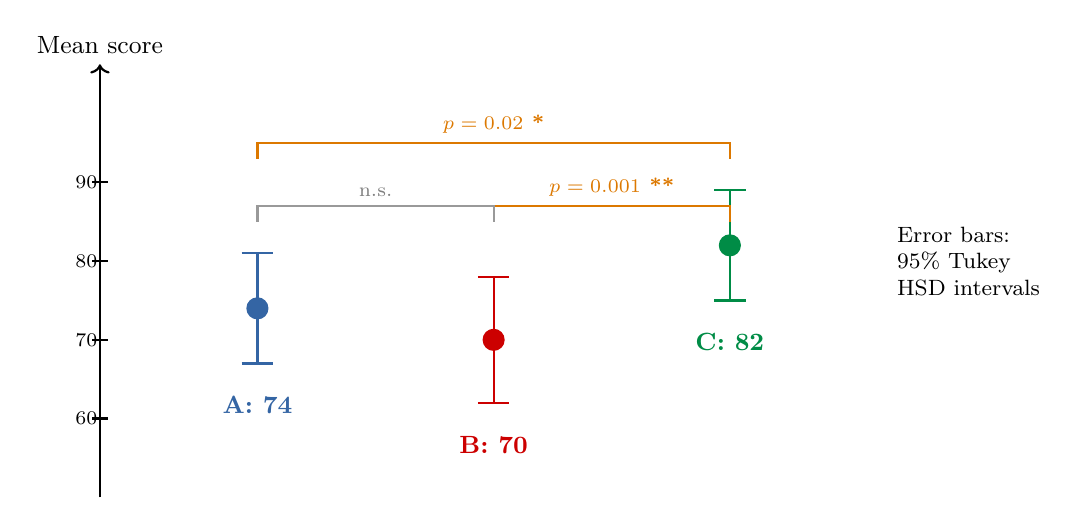
\begin{tikzpicture}
  \draw[thick, ->] (0, 0) -- (0, 5.5) node[above, font=\small] {Mean score};
  \draw[thick] (-0.1, 1) -- (0.1, 1) node[left, font=\scriptsize] {60};
  \draw[thick] (-0.1, 2) -- (0.1, 2) node[left, font=\scriptsize] {70};
  \draw[thick] (-0.1, 3) -- (0.1, 3) node[left, font=\scriptsize] {80};
  \draw[thick] (-0.1, 4) -- (0.1, 4) node[left, font=\scriptsize] {90};

  \fill[popblue] (2, 2.4) circle (4pt);
  \draw[thick, popblue] (2, 1.7) -- (2, 3.1);
  \draw[thick, popblue] (1.8, 1.7) -- (2.2, 1.7);
  \draw[thick, popblue] (1.8, 3.1) -- (2.2, 3.1);
  \node[font=\small\bfseries, popblue, below] at (2, 1.4) {A: 74};

  \fill[sampred] (5, 2.0) circle (4pt);
  \draw[thick, sampred] (5, 1.2) -- (5, 2.8);
  \draw[thick, sampred] (4.8, 1.2) -- (5.2, 1.2);
  \draw[thick, sampred] (4.8, 2.8) -- (5.2, 2.8);
  \node[font=\small\bfseries, sampred, below] at (5, 0.9) {B: 70};

  \fill[paramgreen] (8, 3.2) circle (4pt);
  \draw[thick, paramgreen] (8, 2.5) -- (8, 3.9);
  \draw[thick, paramgreen] (7.8, 2.5) -- (8.2, 2.5);
  \draw[thick, paramgreen] (7.8, 3.9) -- (8.2, 3.9);
  \node[font=\small\bfseries, paramgreen, below] at (8, 2.2) {C: 82};

  \draw[thick, orange1] (2, 4.3) -- (2, 4.5) -- (8, 4.5) -- (8, 4.3);
  \node[font=\scriptsize\bfseries, orange1, above] at (5, 4.5) {$p = 0.02$ *};

  \draw[thick, orange1] (5, 3.5) -- (5, 3.7) -- (8, 3.7) -- (8, 3.5);
  \node[font=\scriptsize\bfseries, orange1, above] at (6.5, 3.7) {$p = 0.001$ **};

  \draw[thick, black!40] (2, 3.5) -- (2, 3.7) -- (5, 3.7) -- (5, 3.5);
  \node[font=\scriptsize, black!50, above] at (3.5, 3.7) {n.s.};

  \node[font=\footnotesize, right, align=left] at (10, 3) {Error bars:\\95\% Tukey\\HSD intervals};
\end{tikzpicture}
\end{center}

\vspace{0.1cm}
\begin{center}
\small If two intervals \textbf{don't overlap}, the difference is significant. Method C is significantly better.
\end{center}
\end{frame}

\begin{frame}
\frametitle{Effect Size: $\eta^2$ (Eta-Squared)}

\begin{center}
\begin{tikzpicture}
  \node[draw=violet1, fill=violet1!5, rounded corners=10pt, text width=10cm, align=center, inner sep=12pt] {
    {\Large $\eta^2 = \dfrac{\text{SS}_{\text{Between}}}{\text{SS}_{\text{Total}}}$}\\[10pt]
    \small Proportion of total variance explained by group membership.
  };
\end{tikzpicture}
\end{center}

\vspace{0.2cm}
\begin{center}
\begin{tikzpicture}[
  cbox/.style={draw, rounded corners=5pt, text width=3cm, align=center, inner sep=6pt, font=\small, minimum height=1.4cm}
]
  \node[cbox, fill=paramgreen!10] at (-4, 0) {\textbf{Small}\\$\eta^2 = 0.01$};
  \node[cbox, fill=orange1!10] at (0, 0) {\textbf{Medium}\\$\eta^2 = 0.06$};
  \node[cbox, fill=warnred!10] at (4, 0) {\textbf{Large}\\$\eta^2 = 0.14$};
\end{tikzpicture}
\end{center}

\vspace{0.2cm}
\small
\textbf{Teaching example:} $\eta^2 = 720/1800 = 0.40$. \textbf{Very large} --- 40\% of score variation is explained by teaching method.

\vspace{0.15cm}
\begin{center}
\fcolorbox{orange1}{orange1!5}{\parbox{10cm}{\centering\footnotesize
  Like Cohen's $d$ for $t$-tests, $\eta^2$ answers: how \textbf{big} is the effect?\\
  A small $p$-value with tiny $\eta^2$ means: real but unimportant.\\[2pt]
  \textbf{Note:} $\eta^2$ is biased upward for small samples. Use $\omega^2$ (omega-squared) for less bias.
}}
\end{center}
\end{frame}

% ============================================================
% PART VII: A/B TESTING
% ============================================================
\section{A/B Testing}

\begin{frame}
\begin{center}
  \vspace{1.5cm}
  {\Huge\bfseries\textcolor{popblue}{Part VII: A/B Testing}}

  \vspace{0.8cm}
  {\large Hypothesis testing meets the real world}
\end{center}
\end{frame}

\begin{frame}
\frametitle{What Is A/B Testing?}

\begin{center}
\begin{tikzpicture}[
  ubox/.style={draw, rounded corners=8pt, text width=4.5cm, align=center, inner sep=10pt, font=\small, minimum height=3cm}
]
  \node[font=\Large\bfseries, popblue] at (0, 3) {Users arrive};
  \draw[->, very thick, popblue] (0, 2.4) -- (0, 1.8);
  \node[diamond, draw=orange1, fill=orange1!10, inner sep=3pt, font=\small\bfseries, align=center] (split) at (0, 1.2) {Random\\split};
  \node[ubox, fill=popblue!8, draw=popblue!50] (ctrl) at (-4, -1.5) {
    {\large\bfseries\textcolor{popblue}{Control (A)}}\\[5pt]
    Current design\\[3pt]
    Blue ``Buy'' button\\[3pt]
    Old checkout flow
  };
  \node[ubox, fill=paramgreen!8, draw=paramgreen!50] (treat) at (4, -1.5) {
    {\large\bfseries\textcolor{paramgreen}{Treatment (B)}}\\[5pt]
    New design\\[3pt]
    Green ``Buy Now!'' button\\[3pt]
    Simplified checkout
  };
  \draw[->, thick] (split) -- node[above left, font=\scriptsize] {50\%} (ctrl);
  \draw[->, thick] (split) -- node[above right, font=\scriptsize] {50\%} (treat);
  \node[draw=violet1!50, fill=violet1!5, rounded corners=5pt, font=\small, text width=10cm, align=center, inner sep=5pt] at (0, -4) {
    \textbf{Measure:} conversion rate, revenue, time on page, \ldots\\
    \textbf{Compare:} Is B significantly better than A?
  };
  \draw[->, thick, violet1] (ctrl) -- (0, -3.3);
  \draw[->, thick, violet1] (treat) -- (0, -3.3);
\end{tikzpicture}
\end{center}
\end{frame}

\begin{frame}
\frametitle{A/B Testing Is Just Hypothesis Testing}

\begin{center}
\begin{tikzpicture}[
  mbox/.style={draw=popblue!40, fill=popblue!3, rounded corners=5pt, text width=12cm, align=left, inner sep=7pt, font=\small}
]
  \node[mbox] at (0, 3.0) {
    \textbf{Step 1 --- Hypothesis:}\;
    $H_0\!: p_B = p_A$ (no difference). \;$H_1\!: p_B \neq p_A$ (or $p_B > p_A$).
  };
  \node[mbox] at (0, 2.0) {
    \textbf{Step 2 --- Sample size:}\;
    Choose $n$ \emph{before} the test using power analysis (L9). Fix $\alpha$, $\beta$, MDE.
  };
  \node[mbox] at (0, 1.0) {
    \textbf{Step 3 --- Randomize:}\;
    Randomly assign users to A or B. Run until planned $n$ is reached.
  };
  \node[mbox] at (0, 0.0) {
    \textbf{Step 4 --- Analyze:}\;
    Two-proportion $z$-test or Welch's $t$-test depending on metric.
  };
  \node[mbox] at (0, -1.0) {
    \textbf{Step 5 --- Decide:}\;
    If $p < \alpha$ \textbf{and} effect is practically significant $\Rightarrow$ ship B.
  };
\end{tikzpicture}
\end{center}

\vspace{0.2cm}
\begin{center}
\fcolorbox{popblue}{popblue!5}{\parbox{10cm}{\centering\small
  \textbf{MDE} = Minimum Detectable Effect.\\
  The smallest improvement worth detecting. Business decides this, not statistics.
}}
\end{center}
\end{frame}

\begin{frame}
\frametitle{Sample Size Planning for A/B Tests}
\framesubtitle{For comparing two proportions ($p_A$ vs $p_B$)}

\begin{center}
\begin{tikzpicture}
  \node[draw=popblue, fill=popblue!5, rounded corners=10pt, text width=10cm, align=center, inner sep=10pt] {
    {\Large $n = \dfrac{(z_{\alpha/2} + z_\beta)^2 \cdot (p_A(1-p_A) + p_B(1-p_B))}{(p_B - p_A)^2}$}\\[8pt]
    \small $n$ = per group. This is the two-proportion version from L9's power formula.
  };
\end{tikzpicture}
\end{center}

\vspace{0.2cm}
\small
\textbf{Example:} Baseline conversion $p_A = 5\%$. Want to detect $p_B = 6\%$ (MDE $= 1$ pp).\\
$\alpha = 0.05$, power $= 80\%$ ($z_{0.025} = 1.96$, $z_{0.20} = 0.84$).

$$n = \frac{(1.96 + 0.84)^2 \times (0.05 \times 0.95 + 0.06 \times 0.94)}{(0.01)^2} = \frac{7.84 \times 0.1039}{0.0001} \approx \mathbf{8{,}146}$$

\vspace{0.1cm}
\begin{center}
\fcolorbox{warnred}{warnred!5}{\parbox{10cm}{\centering\small
  Need $\sim$\textbf{8,000 users per group} (16,000 total) to detect a 1\% lift in conversion.\\
  Small effects need big samples. This is why A/B tests take weeks.
}}
\end{center}
\end{frame}

\begin{frame}
\frametitle{A/B Test Example: Button Color}

\small
\textbf{Setup:} $n_A = 5{,}000$ (blue button), $n_B = 5{,}000$ (green button).\\
Results: $k_A = 230$ conversions ($\hat{p}_A = 4.6\%$), $k_B = 275$ ($\hat{p}_B = 5.5\%$).

\vspace{0.15cm}
\textbf{Pooled proportion:} $\hat{p} = (230 + 275)/(5000 + 5000) = 0.0505$.

$$Z = \frac{0.055 - 0.046}{\sqrt{0.0505 \times 0.9495 \times (1/5000 + 1/5000)}} = \frac{0.009}{0.0044} = 2.05$$

\vspace{0.1cm}
$p\text{-value} = 2(1 - \Phi(2.05)) = 0.040 < 0.05$: \textbf{reject} $H_0$.

\vspace{0.15cm}
\begin{center}
\begin{tikzpicture}
  \fill[popblue!50] (0, 0) rectangle (2.3, 2);
  \fill[paramgreen!50] (3.5, 0) rectangle (5.8+0.45, 2);
  \node[font=\large\bfseries, white] at (1.15, 1) {4.6\%};
  \node[font=\large\bfseries, white] at (4.625+0.225, 1) {5.5\%};
  \node[font=\small\bfseries, popblue] at (1.15, -0.3) {Control (Blue)};
  \node[font=\small\bfseries, paramgreen] at (4.625+0.225, -0.3) {Treatment (Green)};
  \node[draw=orange1, fill=orange1!10, rounded corners=4pt, font=\small\bfseries, inner sep=5pt, align=center] at (9, 1) {
    $+$19.6\% relative lift\\
    $p = 0.040$
  };
\end{tikzpicture}
\end{center}

\vspace{0.05cm}
\small\textbf{Decision:} Statistically significant. +19.6\% relative lift is practically meaningful. Ship the green button.

\vspace{0.02cm}
{\scriptsize\textcolor{gray}{\textbf{Absolute vs relative:} MDE and sample size formulas use \emph{absolute} differences (0.9 pp here). Lift is usually reported \emph{relative} ($0.009/0.046 = 19.6\%$). Don't confuse the two!}}
\end{frame}

% ============================================================
% PART VIII: A/B PITFALLS
% ============================================================
\section{A/B Testing Pitfalls}

\begin{frame}
\begin{center}
  \vspace{1.5cm}
  {\Huge\bfseries\textcolor{popblue}{Part VIII: A/B Testing Pitfalls}}

  \vspace{0.8cm}
  {\large The theory is simple. The practice is full of traps.}
\end{center}
\end{frame}

\begin{frame}
\frametitle{Pitfall 1: Peeking (The Most Common Mistake)}

\begin{center}
\begin{tikzpicture}
  \begin{axis}[
    width=10cm, height=4.5cm,
    xlabel={Day},
    ylabel={$p$-value},
    xmin=0, xmax=30,
    ymin=0, ymax=0.3,
    grid=major, grid style={gray!15},
    every axis plot/.style={thick, no markers},
    clip=false
  ]
    \addplot[popblue, thick] coordinates {
      (1, 0.25) (3, 0.18) (5, 0.12) (7, 0.08) (9, 0.04) (10, 0.03)
      (12, 0.06) (14, 0.09) (16, 0.07) (18, 0.11) (20, 0.13)
      (22, 0.10) (24, 0.08) (26, 0.07) (28, 0.065) (30, 0.07)
    };
    \draw[thick, dashed, warnred] (axis cs:0, 0.05) -- (axis cs:30, 0.05);
    \node[font=\scriptsize, warnred, right] at (axis cs:30, 0.05) {$\alpha = 0.05$};
    \draw[thick, ->, sampred] (axis cs:10, 0.12) -- (axis cs:10, 0.05);
    \node[font=\scriptsize\bfseries, sampred, above] at (axis cs:10, 0.12) {``It's significant! Ship it!''};
    \node[font=\scriptsize, paramgreen, above] at (axis cs:30, 0.09) {Final $p = 0.07$ (not sig.)};
  \end{axis}
\end{tikzpicture}
\end{center}

\vspace{0.1cm}
\begin{center}
\fcolorbox{warnred}{warnred!5}{\parbox{11cm}{\centering\small
  \textbf{If you check daily and stop when $p < 0.05$,} the true false positive rate\\
  can be \textbf{26\%} or higher, not 5\%. The $p$-value fluctuates --- early dips are noise.\\[3pt]
  \textbf{Fix:} Decide sample size \emph{before} the test. Don't peek.
}}
\end{center}
\end{frame}

\begin{frame}
\frametitle{Pitfall 2: Too Many Metrics}

\begin{center}
\begin{tikzpicture}[
  mbox/.style={draw=popblue!40, fill=popblue!3, rounded corners=5pt, text width=5cm, align=center, inner sep=6pt, font=\small}
]
  \node[mbox] at (-3.8, 1.8) {Conversion rate};
  \node[mbox] at (3.8, 1.8) {Revenue per user};
  \node[mbox] at (-3.8, 0.6) {Time on page};
  \node[mbox] at (3.8, 0.6) {Bounce rate};
  \node[mbox] at (-3.8, -0.6) {Pages per session};
  \node[mbox] at (3.8, -0.6) {Cart abandonment};
  \node[mbox, draw=warnred!60, fill=warnred!8] at (-3.8, -1.8) {Newsletter signup};
  \node[mbox] at (3.8, -1.8) {Customer satisfaction};
\end{tikzpicture}
\end{center}

\vspace{0.15cm}
\begin{center}
\small
Test 8 metrics at $\alpha = 0.05$: $P(\text{at least one false positive}) = 1 - 0.95^8 = 0.34$.

\vspace{0.1cm}
\fcolorbox{orange1}{orange1!5}{\parbox{10cm}{\centering\footnotesize
  \textbf{Fix:} Pick \textbf{one primary metric} before the test. Others are exploratory.\\
  If you must test many, apply Bonferroni or BH correction (L9).
}}
\end{center}
\end{frame}

\begin{frame}
\frametitle{More Pitfalls}

\begin{center}
\begin{tikzpicture}[
  pbox/.style={draw=warnred!50, fill=warnred!5, rounded corners=5pt, text width=11.5cm, align=left, inner sep=7pt, font=\small}
]
  \node[pbox] at (0, 2.8) {
    \textbf{3.\ Novelty \& primacy effects:}
    Users click the new thing \emph{because} it's new, not because it's better.
    Effect fades after 1--2 weeks.
    \textcolor{paramgreen}{\textbf{Fix:}} run test long enough (2+ weeks).
  };
  \node[pbox] at (0, 1.2) {
    \textbf{4.\ Simpson's paradox:}
    Overall B wins, but A wins in \emph{every} segment (mobile, desktop, tablet).
    Caused by unequal traffic mix.
    \textcolor{paramgreen}{\textbf{Fix:}} stratified randomization.
  };
  \node[pbox] at (0, -0.4) {
    \textbf{5.\ Interference / network effects:}
    If user A's experience affects user B (social networks, marketplaces),
    standard randomization breaks.
    \textcolor{paramgreen}{\textbf{Fix:}} cluster randomization (by region, by network cluster).
  };
  \node[pbox] at (0, -2.0) {
    \textbf{6.\ Survivorship bias:}
    Only analyzing users who \emph{completed} the funnel.
    Ignoring those who dropped off.
    \textcolor{paramgreen}{\textbf{Fix:}} intent-to-treat analysis.
  };
\end{tikzpicture}
\end{center}
\end{frame}

% ============================================================
% PART IX: BIG PICTURE
% ============================================================
\section{The Big Picture}

\begin{frame}
\frametitle{ANOVA and A/B Testing: Same Core, Different Worlds}

\begin{center}
\begin{tikzpicture}
  \node[inner sep=0pt] {
    \small
    \begin{tabular}{l|p{5cm}|p{5cm}}
       & \textbf{ANOVA} & \textbf{A/B Testing} \\
      \hline
      \textbf{Setting} & Science, medicine, education & Tech, product, marketing \\
      \textbf{Groups} & 2+ (often 3--5) & Usually 2 (A vs B) \\
      \textbf{Design} & Controlled experiment & Online randomized experiment \\
      \textbf{Metric} & Continuous (scores, times) & Often proportions (conversion) \\
      \textbf{Analysis} & $F$-test + post-hoc & $z$-test or $t$-test \\
      \textbf{Pitfalls} & Assumptions, multiple comp. & Peeking, novelty, interference \\
      \textbf{Effect size} & $\eta^2$ & Relative lift (\%) \\
    \end{tabular}
  };
\end{tikzpicture}
\end{center}

\vspace{0.3cm}
\begin{center}
\fcolorbox{popblue}{popblue!5}{\parbox{10cm}{\centering\small
  \textbf{Both are hypothesis tests.} ANOVA generalizes to $k$ groups.\\
  A/B testing adds the engineering of randomization, sample size, and deployment.\\
  An A/B test with 3+ variants is literally ANOVA (sometimes called A/B/n testing).
}}
\end{center}
\end{frame}

\begin{frame}
\frametitle{When To Use What}

\begin{center}
\begin{tikzpicture}[
  tbox/.style={draw=popblue!50, fill=popblue!3, rounded corners=5pt, text width=12cm, align=left, inner sep=7pt, font=\small}
]
  \node[tbox] at (0, 2.4) {
    \textbf{2 groups, continuous metric:}\;
    Welch's $t$-test (or Mann--Whitney if non-Normal).
  };
  \node[tbox] at (0, 1.4) {
    \textbf{2 groups, proportions:}\;
    Two-proportion $z$-test. The classic A/B test.
  };
  \node[tbox] at (0, 0.4) {
    \textbf{$k \geq 3$ groups, continuous:}\;
    One-way ANOVA $\to$ post-hoc (Tukey). Or Kruskal--Wallis if non-Normal.
  };
  \node[tbox] at (0, -0.6) {
    \textbf{$k \geq 3$ groups, proportions:}\;
    $\chi^2$ test of homogeneity ($= \chi^2$ independence test on proportions).
  };
  \node[tbox] at (0, -1.6) {
    \textbf{Two categorical variables, association:}\;
    $\chi^2$ test of independence.
  };
\end{tikzpicture}
\end{center}
\end{frame}

% ============================================================
\section{Summary}

\begin{frame}
\frametitle{Summary: Lectures 10--11}
\begin{center}
\begin{tikzpicture}[
  sbox/.style={draw=popblue!60, fill=popblue!5, rounded corners=4pt, text width=12cm, minimum height=0.5cm, align=left, inner sep=5pt, font=\small}
]
  \node[sbox] at (0, 3.6) {\textbf{$t$-tests:} one-sample, paired, Welch's two-sample. Workhorses of inference.};
  \node[sbox] at (0, 2.8) {\textbf{$\chi^2$ tests:} GoF and independence. Statistic = sum of squared standardized errors.};
  \node[sbox] at (0, 2.0) {\textbf{Nonparametric:} Mann--Whitney, Wilcoxon when normality fails.};
  \node[sbox] at (0, 1.2) {\textbf{LRT:} all of the above are special cases. $-2\log\Lambda \dot\sim \chi^2_k$ (Wilks).};
  \node[sbox] at (0, 0.4) {\textbf{ANOVA:} $F = \text{MS}_\text{B}/\text{MS}_\text{W}$. Single test for $k$ group means.};
  \node[sbox] at (0, -0.4) {\textbf{Post-hoc:} Tukey HSD or Bonferroni once ANOVA rejects.};
  \node[sbox] at (0, -1.2) {\textbf{Effect size:} $\eta^2$, Cohen's $d$. ``Real'' $\neq$ ``meaningful''.};
  \node[sbox] at (0, -2.0) {\textbf{A/B testing:} same machinery, plus engineering: randomization, sample size, deployment.};
  \node[sbox] at (0, -2.8) {\textbf{Pitfalls:} peeking, too many metrics, novelty, Simpson's, interference.};
\end{tikzpicture}
\end{center}
\end{frame}

% ============================================================
\section{Practical}

\begin{frame}
\frametitle{Practical: Classical Tests}
\begin{center}
\begin{tikzpicture}
  \node[draw=popblue, fill=popblue!3, rounded corners=10pt, text width=12cm, align=left, inner sep=12pt] {
    \begin{enumerate}\setlength{\itemsep}{4pt}
      \item \textbf{One-sample $t$-test:}
        \begin{itemize}\setlength{\itemsep}{1pt}
          \item Coffee shop data ($n{=}25$, $\bar{X}{=}345$, $S{=}10$, $\mu_0{=}350$)
          \item Compute $T$, find $p$ from $t$-table, verify with \texttt{scipy.stats.ttest\_1samp}
        \end{itemize}
      \item \textbf{Paired $t$-test:}
        \begin{itemize}\setlength{\itemsep}{1pt}
          \item Blood pressure before/after. Compute by hand and with \texttt{ttest\_rel}
        \end{itemize}
      \item \textbf{Welch's $t$-test:}
        \begin{itemize}\setlength{\itemsep}{1pt}
          \item Teaching method data. Use \texttt{ttest\_ind(equal\_var=False)}
          \item Compare $p$ with the permutation test from L9
        \end{itemize}
      \item \textbf{$\chi^2$ independence test:}
        \begin{itemize}\setlength{\itemsep}{1pt}
          \item Smoking/cancer $2 \times 2$ table. Compute by hand
          \item Verify with \texttt{scipy.stats.chi2\_contingency}
        \end{itemize}
    \end{enumerate}
  };
\end{tikzpicture}
\end{center}
\end{frame}

\begin{frame}
\frametitle{Practical: ANOVA \& A/B Testing in Python}
\begin{center}
\begin{tikzpicture}
  \node[draw=popblue, fill=popblue!3, rounded corners=10pt, text width=12cm, align=left, inner sep=12pt] {
    \begin{enumerate}\setlength{\itemsep}{4pt}
      \item \textbf{One-way ANOVA:}
        \begin{itemize}\setlength{\itemsep}{1pt}
          \item Generate 3 groups with \texttt{np.random.normal} (same vs different means)
          \item Run \texttt{scipy.stats.f\_oneway}. Check $F$ and $p$
          \item Post-hoc with \texttt{statsmodels.stats.multicomp.pairwise\_tukeyhsd}
        \end{itemize}
      \item \textbf{Assumptions check:}
        \begin{itemize}\setlength{\itemsep}{1pt}
          \item Levene's test: \texttt{scipy.stats.levene}
          \item Kruskal--Wallis: \texttt{scipy.stats.kruskal}
        \end{itemize}
      \item \textbf{A/B test simulation:}
        \begin{itemize}\setlength{\itemsep}{1pt}
          \item Simulate $n$ Bernoulli trials for A and B. Run $z$-test
          \item Repeat 10,000 times. Check: is the rejection rate $\approx \alpha$?
        \end{itemize}
      \item \textbf{Peeking simulation:}
        \begin{itemize}\setlength{\itemsep}{1pt}
          \item Simulate with $p_A = p_B$ (no effect). Check daily
          \item Count how often $p < 0.05$ at \emph{any} day. Compare to 5\%
        \end{itemize}
    \end{enumerate}
  };
\end{tikzpicture}
\end{center}
\end{frame}

\begin{frame}
\frametitle{Homework}
\small
\begin{enumerate}\setlength{\itemsep}{4pt}
  \item A manufacturer claims mean weight is 500\,g. Sample $n = 16$: $\bar{X} = 495$, $S = 8$.\\
    Test at $\alpha = 0.05$. Compute the 95\% CI. Does it contain 500?

  \item 12 runners' times (s) before and after training:\\
    Before: 58.2, 57.1, 60.3, 55.8, 59.6, 62.1, 56.4, 61.2, 58.7, 57.5, 60.8, 59.3.\\
    After: 56.1, 55.8, 58.7, 54.2, 57.3, 59.8, 55.1, 59.0, 56.4, 56.0, 58.2, 57.1.\\
    (a) Paired $t$-test. (b) Unpaired $t$-test on the same data. Why does the $p$-value change?

  \item Survey of 300 people on preferred transport: bus 90, metro 120, car 60, bicycle 30.\\
    Test whether preferences are equally distributed ($\chi^2$ goodness-of-fit).

  \item Study method (group/solo) vs exam result (pass/fail): Group+pass 70, Group+fail 30,\\
    Solo+pass 55, Solo+fail 45. Test independence at $\alpha = 0.05$.

  \item Startup salaries (thousands): Team A: 120, 45, 38, 200, 52. Team B: 55, 62, 48, 70, 58.\\
    (a) Why is a $t$-test problematic here? (b) Use Mann--Whitney $U$ (\texttt{scipy.stats.mannwhitneyu}).

  \item Three fertilizers tested on plant height ($n = 15$ per group):\\
    A: $\bar{X}_1 = 22.1$, $S_1 = 3.2$. \;B: $\bar{X}_2 = 25.4$, $S_2 = 3.5$. \;C: $\bar{X}_3 = 24.8$, $S_3 = 2.9$.\\
    (a) Compute $\text{SS}_\text{B}$, $\text{SS}_\text{W}$, $F$. (b) Test at $\alpha = 0.05$ ($F_{2,42,0.05} = 3.22$).\\
    (c) Compute $\eta^2$. (d) Which fertilizer is best? (Use Bonferroni with $\alpha/3$.)

  \item E-commerce site tests two checkout flows ($n = 3{,}000$ per group):\\
    Control: 156 conversions. \;Treatment: 189 conversions.\\
    (a) Compute $\hat{p}_A$, $\hat{p}_B$, $Z$, $p$-value. (b) Significant at $\alpha = 0.05$?\\
    (c) Relative lift? (d) Sample size needed for a 0.5\% absolute lift?

  \item \textbf{Peeking simulation} (Python):
    Simulate 1,000 A/B tests where $p_A = p_B = 0.05$ (no true effect), $n = 5{,}000$ per group.
    For each test, compute the $p$-value after every 500 users.
    What fraction show $p < 0.05$ at \emph{any} checkpoint? Compare to $\alpha = 0.05$.

  \item A 3-way A/B/C test: $n_A = 1000$, $k_A = 48$; $n_B = 1000$, $k_B = 55$; $n_C = 1000$, $k_C = 62$.\\
    Test using $\chi^2$ test of homogeneity. Then do pairwise $z$-tests with Bonferroni.
\end{enumerate}
\end{frame}

\begin{frame}
\frametitle{Recommended Resources}

\footnotesize
\begin{center}
\begin{tikzpicture}[
  rbox/.style={draw=popblue!40, fill=popblue!3, rounded corners=5pt, text width=12.5cm, align=left, inner sep=6pt, font=\footnotesize}
]
  \node[rbox] at (0, 2.8) {
    \textbf{\textcolor{popblue}{Interactive: Seeing Theory --- Brown University}}\\[1pt]
    \scriptsize\texttt{seeing-theory.brown.edu/frequentist-inference} --- $t$-tests, $\chi^2$, regression with sliders.
  };
  \node[rbox] at (0, 1.6) {
    \textbf{\textcolor{popblue}{Video: StatQuest}}\\[1pt]
    \scriptsize ``$t$-Tests Explained'', ``Chi-Square Tests'', ``ANOVA'', ``A/B Testing''. Clear and concise.
  };
  \node[rbox] at (0, 0.4) {
    \textbf{\textcolor{popblue}{Reading: Wasserman, ``All of Statistics'' --- Ch.\ 10--11}}\\[1pt]
    \scriptsize Hypothesis testing, LRT framework, $t$-tests, $\chi^2$ tests. Concise and rigorous.
  };
  \node[rbox] at (0, -0.8) {
    \textbf{\textcolor{popblue}{Reading: Kohavi, Tang \& Xu --- ``Trustworthy Online Controlled Experiments''}}\\[1pt]
    \scriptsize The definitive book on A/B testing from Microsoft researchers.
  };
  \node[rbox] at (0, -2.0) {
    \textbf{\textcolor{popblue}{Blog: Evan Miller --- ``How Not to Run an A/B Test''}}\\[1pt]
    \scriptsize Classic post on the peeking problem. Required reading for anyone running A/B tests.
  };
  \node[rbox] at (0, -3.2) {
    \textbf{\textcolor{popblue}{Python: \texttt{scipy.stats} + \texttt{statsmodels}}}\\[1pt]
    \scriptsize \texttt{ttest\_*}, \texttt{chi2\_contingency}, \texttt{mannwhitneyu}, \texttt{wilcoxon}, \texttt{f\_oneway}, \texttt{kruskal}, \texttt{levene}, \texttt{pairwise\_tukeyhsd}, \texttt{proportions\_ztest}.
  };
\end{tikzpicture}
\end{center}
\end{frame}

\begin{frame}
\begin{center}
  {\Huge\bfseries\textcolor{popblue}{Questions?}}

  \vspace{1cm}

  {\large Next: Lecture~12 --- Regression inference}
\end{center}
\end{frame}

\end{document}
